% JUTIF manuscript -- LaTeX version of JUTIF_Manuscript_FedXPalm_B1B2.docx
% Build: latexmk -pdf manuscript.tex   (or: pdflatex manuscript.tex, run twice for refs)
% Or just open this project on Overleaf (New Project > Upload Project) -- no local
% LaTeX install needed, Overleaf compiles it for you. See README.md in this folder.
%
% Content transcribed 1:1 from the .docx in this folder; [TODO: ...] markers
% preserved verbatim -- do NOT fill them with guesses, see docs/thesis/NOTES_FOR_RACHMA.md.
%
% Running header/footer, margins, heading style, line spacing, and paragraph
% indent below all mirror the REAL JUTIF-Template.docx (word/header1.xml,
% word/footer1.xml, word/styles.xml pStyle definitions JUDUL/AUTHOR/BODYPARAGRAP/
% 3METODE/4PEMBAHASAN/SUBJUDUL, word/document.xml sectPr) -- confirmed against
% JUTIFTemplate.docx directly, not inferred from the manuscript body text alone:
%  - pgMar: top=1418 right=1418 bottom=1134 left=1418 twips = 2.5/2.5/2.0/2.5 cm
%    (top pushed out further below to fit the 3-line header block, matching
%    what Word itself does when header content exceeds the nominal header gap)
%  - BODYPARAGRAP: line=276/240=1.15 line spacing, firstLine indent=624 twips=1.1cm,
%    after=0 (no extra paragraph skip -- indent-style, not block-style)
%  - Section headings (3METODE/4PEMBAHASAN/5KESIMPULAN, based on Heading1): bold,
%    ALL CAPS (w:caps), 12pt, NOT numbered (no numPr on these styles)
%  - SUBJUDUL (sub-headings): bold, 12pt, normal case, also not numbered
%  - JUDUL (title): bold, 14pt, centered  |  AUTHOR: bold, 10pt, centered
% Because headings are unnumbered in the real template, all inline "Section N"
% cross-references were rewritten as plain subsection names instead of \ref{}
% (an unnumbered \section has no number for \ref to print).
\documentclass[11pt]{article}

\usepackage[a4paper,top=3.4cm,bottom=2cm,left=2.5cm,right=2.5cm,headheight=62pt,headsep=14pt]{geometry}
\usepackage{mathptmx}          % Times New Roman-equivalent text+math font, per JUTIF checklist item "Times New Roman 11pt"
\usepackage[T1]{fontenc}
\usepackage{graphicx}
\usepackage{booktabs}
\usepackage{caption}
\usepackage{amsmath}
\usepackage{xcolor}
\usepackage{fancyhdr}
\usepackage{titlesec}
\usepackage{float}             % [H] below pins each figure/table exactly where it's declared in the
                                % source instead of letting LaTeX float it onto a later page, which
                                % kept landing figures in the middle of unrelated paragraphs
\usepackage[colorlinks=true,linkcolor=blue,citecolor=blue,urlcolor=blue]{hyperref}
\usepackage[english]{babel}

\newcommand{\todo}[1]{\textcolor{red}{[TODO: #1]}}
% Fields assigned by the JUTIF editorial office only upon submission/acceptance
% (volume, issue, page range, DOI, review-timeline dates) -- genuinely unknown
% pre-submission, not an author-side omission, so styled as a plain placeholder
% rather than the loud red \todo used for actual outstanding author work.
\newcommand{\editorialtbd}{\textit{TBD}}

% --- Body text: 1.15 line spacing, 1.1cm first-line indent, no paragraph skip
% (BODYPARAGRAP style) ---
\linespread{1.15}
\setlength{\parindent}{1.1cm}
\setlength{\parskip}{0pt}

% --- Section headings: unnumbered, bold, ALL CAPS, 12pt (3METODE/4PEMBAHASAN/
% 5KESIMPULAN styles); sub-headings: unnumbered, bold, normal case, 12pt (SUBJUDUL) ---
\setcounter{secnumdepth}{-1}
\titleformat{\section}{\normalfont\fontsize{12}{14}\bfseries\MakeUppercase}{}{0pt}{}
\titlespacing*{\section}{0pt}{0.35cm}{0.18cm}
\titleformat{\subsection}{\normalfont\fontsize{12}{14}\bfseries}{}{0pt}{}
\titlespacing*{\subsection}{0pt}{0.35cm}{0.18cm}

% --- JUTIF running header/footer (mirrors header1.xml / footer1.xml) ---
\pagestyle{fancy}
\fancyhf{}
\renewcommand{\headrulewidth}{0.5pt}
\renewcommand{\footrulewidth}{0pt}
\fancyhead[C]{%
  \small
  \begin{tabular*}{\textwidth}{@{\extracolsep{\fill}}p{0.55\textwidth}p{0.4\textwidth}}
    \textbf{Jurnal Teknik Informatika (JUTIF)} & Vol. \editorialtbd, No. \editorialtbd, \editorialtbd\ \editorialtbd, Page. \editorialtbd \\
    P-ISSN: 2723-3863 & https://jutif.if.unsoed.ac.id \\
    E-ISSN: 2723-3871 & DOI: \editorialtbd\ (assigned upon acceptance)
  \end{tabular*}%
}
\fancyfoot[C]{\thepage}

\title{\vspace{-1.5em}\fontsize{14}{17}\selectfont\bfseries Multi-Seed Reproducibility and Convergence Stability of Non-IID Federated YOLO11n for Oil Palm Fresh Fruit Bunch Detection}
\author{
  \bfseries\fontsize{10}{12}\selectfont Rachma Dianty$^{*1}$, Favian Dewanta$^{2}$, Teddy Surya Gunawan$^{3}$ \\
  \normalfont\small ($^{*}$ = corresponding author) \\
  \small $^{1,2}$Master of Electrical-Telecommunication Engineering, School of Electrical Engineering, Telkom University, Bandung, Indonesia \\
  \small $^{3}$Department of Electrical and Computer Engineering, International Islamic University Malaysia, Kuala Lumpur, Malaysia \\
  \small Email: rachmadiantyy@gmail.com$^{1}$ (only email for corresponding author) \\
  \small Received: \editorialtbd; Revised: \editorialtbd; Accepted: \editorialtbd; Published: \editorialtbd
}
\date{}

\begin{document}
\maketitle
\thispagestyle{fancy}

\begin{abstract}
\noindent
Federated learning (FL) enables collaborative model training across distributed data holders without centralizing raw images, which is attractive for oil palm plantation operators facing data-sharing and bandwidth constraints. However, FL deployments in agricultural computer vision are frequently reported from a single training run, leaving open how reproducible their reported performance is under independent stochastic training realizations. This study evaluates the reproducibility and convergence stability of Federated Averaging (FedAvg) for six-class oil palm fresh fruit bunch (FFB) ripeness detection using YOLO11n with Group Normalization, under a fixed Non-IID client partition (Dirichlet $\alpha=0.5$, K=4 simulated clients, training-image share ranging 8.67\%--59.36\% per client) on a leakage-free, source-group-aware dataset split (8,937 training / 826 validation / 1,051 held-out test images). Training was replicated across three independent seeds (42, 123, 2026) over 40 communication rounds each. Validation mAP50 converged to a stable mean of 0.8775 (SD = 0.0157) across seeds, but the best-validation checkpoint occurred at markedly different rounds (9, 11, and 40, respectively), indicating that outcome-level reproducibility does not imply trajectory-level reproducibility. A centralized reference model, evaluated once on the held-out test split, achieved mAP50 = 0.8820 (mAP50-95 = 0.7309), which is reported descriptively alongside -- not as a matched comparison against -- the federated validation results. These findings suggest that multi-seed reporting is necessary to characterize federated training behavior under Non-IID partitions, and that checkpoint-selection policy should account for seed-dependent convergence speed. A subsequent matched held-out-test evaluation of all three federated checkpoints (mean mAP50 = 0.8031, SD = 0.0319) revealed a centralized-versus-federated gap (0.0789) substantially larger than the validation-based indicative comparison (0.0045) suggested, and a cross-seed spread roughly twice that observed on validation -- underscoring that validation-only reproducibility reporting can understate both the utility gap and the outcome variability that a matched held-out evaluation reveals.

\medskip
\noindent\textbf{Keywords:} Federated Learning; Non-IID Data; Reproducibility; Convergence Stability; Oil Palm Ripeness Detection; YOLO11.

\medskip
\noindent\footnotesize This work is an open access article licensed under a Creative Commons Attribution 4.0 International License.
\end{abstract}

\section{Introduction}

Precise, non-destructive assessment of fresh fruit bunch (FFB) ripeness is a long-standing operational problem in oil palm cultivation, since harvesting decisions made from ripeness stage directly affect oil extraction rate and downstream yield \cite{suharjito2021,goh2025}. Because ripeness assessment in commercial operations is still predominantly performed through manual visual inspection, harvesting decisions can be inconsistent across harvesters and across observation conditions such as lighting and viewing angle, which in turn motivates automated, image-based ripeness assessment as a means of supporting more objective and repeatable harvesting decisions \cite{suharjito2021,goh2025}. Deep-learning-based object detectors, and in particular the YOLO family, have been widely adopted for this task because they combine real-time inference speed with competitive detection accuracy \cite{redmon2016,jocher2024}. In practical deployments, FFB image data are frequently distributed across multiple sources (e.g., different harvesting sites, collection batches, or partner organizations) rather than residing in a single centralized repository. Centralizing such data for model training raises data-sharing and logistical concerns, which motivates the use of Federated Learning (FL) \cite{mcmahan2017fedavg,konecny2016} as a means of collaborative model training without transmitting raw images to a central server.

FL allows multiple clients to collaboratively train a shared model by exchanging model updates rather than raw data \cite{mcmahan2017fedavg}. It is important to note that FL, by itself, does not constitute a formal privacy guarantee: model updates and gradients can still leak information about the underlying training samples \cite{zhu2019,zhao2020}. Formal guarantees require mechanisms such as Differential Privacy (DP-SGD), which are outside the scope of the present study and are noted only briefly as future work in the Discussion section. The property this study relies on is narrower and purely logistical: FL avoids the specific operational requirement of centralizing raw plantation imagery on a single server.

A separate, and for deployment purposes equally important, question is \emph{reproducibility}. Because FedAvg optimization under Non-IID client data is a stochastic process influenced by local data shuffling order, augmentation sampling, minibatch composition, optimizer dynamics, and potentially nondeterministic GPU operations, a single federated training run cannot by itself establish whether a reported performance level is a stable, repeatable outcome or an artifact of one favorable stochastic trajectory. (Client participation itself is not a source of stochasticity in this study: all four clients participate in every communication round, per the \emph{Federated Partition} subsection below.) This distinction matters operationally: a practitioner deciding whether to deploy a federated-trained model needs to know not only its peak achievable performance, but whether that performance -- and the number of communication rounds required to reach it -- is consistent across independent training runs.

\subsection*{Research Gap}
Prior work has separately examined YOLO-based object detection for oil palm FFB ripeness \cite{lai2022,suharjito2021,suharjito2023dataset,asrol2023,goh2025} and Federated Learning for visual classification and detection under Non-IID data \cite{mcmahan2017fedavg,hsu2019,kairouz2021}. However, federated learning studies in agricultural computer vision typically report results from a single training run, without characterizing performance variance or convergence-trajectory variance across independent stochastic seeds. This gap is consequential because single-run reports cannot distinguish a reproducible training regime from a favorable outlier run, which is precisely the distinction this study is designed to test. This study does not claim to be the first application of Federated Learning to oil palm imagery or the first use of YOLO for FFB ripeness classification; rather, it establishes a multi-seed empirical characterization of reproducibility and convergence behavior for this specific task, architecture, and federation setting.

\subsection*{Research Question}
The primary research question addressed in this study is: under a fixed Non-IID client partition (Dirichlet $\alpha=0.5$, K=4), how reproducible is FedAvg-trained YOLO11n's detection performance across independent stochastic training seeds, and how consistent is its convergence behavior across communication rounds?

This is examined through three supporting questions: (i) does peak validation performance remain stable across training seeds even when the communication round at which that peak occurs varies substantially; (ii) how does FedAvg convergence behave under the observed client data-quantity imbalance (8.67\%--59.36\% of training images per client) and sample-weighted aggregation, noting that this study describes convergence behavior under a single fixed partition and does not, by itself, establish a causal effect of imbalance without a balanced-partition control; and (iii) is federated training's per-class detection stability consistent with its global mAP stability, or do specific ripeness classes show disproportionate inter-seed variance that a single aggregate metric would hide.

\subsection*{Contributions}
(1) A multi-seed ($n=3$) empirical evaluation of FedAvg under a fixed Non-IID Dirichlet partition ($\alpha=0.5$, K=4) for six-class oil palm FFB ripeness detection using YOLO11n, reporting outcome-level reproducibility (mean validation mAP50 = 0.8775, SD = 0.0157). (2) A convergence-trajectory analysis across 40 communication rounds per seed, showing that the best-validation checkpoint round varies substantially across seeds (round 9, 11, and 40) despite comparable peak validation performance -- distinguishing outcome reproducibility from trajectory reproducibility. (3) A quantitative characterization of federated client heterogeneity at both the quantity level (training-image count: 8.67\%--59.36\% share across four simulated clients, coefficient of variation $\approx 0.82$) and the class level (per-client, per-class bounding-box distribution, normalized entropy, and Jensen--Shannon divergence from the global distribution), showing that the two forms of heterogeneity are not aligned in this partition and motivating discussion of sample-weighted FedAvg aggregation dynamics. (4) A leakage-audited, source-group-aware train/validation/held-out-test protocol that separates the reproducibility analysis (validation split, multi-seed) from a single locked centralized reference point (held-out test split). (5) An architectural adaptation (Batch Normalization to Group Normalization throughout) applied consistently across all training configurations, reported here as a design choice compatible with small Non-IID per-client batches, not as an empirically demonstrated performance improvement. Centralized training (B1) is retained strictly as a single reference point, not as a co-equal contribution.

\subsection*{Related Work}
\textbf{Oil palm FFB detection and grading.} Deep-learning-based detection of oil palm FFB ripeness has predominantly used one-stage object detectors, particularly YOLO-based architectures built on convolutional backbones such as CSPNet \cite{wang2020cspnet} and residual networks \cite{he2016}, for their real-time performance \cite{lai2022,suharjito2021,suharjito2023dataset,asrol2023,goh2025}. Lai et al.\ applied YOLOv4 to real-time ripe-bunch detection in plantation settings \cite{lai2022}, while Suharjito et al.\ targeted mobile-device deployment for FFB ripeness classification \cite{suharjito2021}; a recent review notes that most reported systems remain single-site, centrally trained models \cite{goh2025}.

\textbf{Federated learning for computer vision and object detection.} FedAvg \cite{mcmahan2017fedavg} remains the standard aggregation baseline for federated visual learning. Federated learning under Non-IID client data has been studied for general vision classification tasks \cite{hsu2019,kairouz2021}. Within agriculture specifically, federated learning has more commonly been applied to image classification -- for example, crop disease classification across multiple clients \cite{kabala2023} -- than to object detection; a federated, multi-seed, Non-IID evaluation of an object detector for agricultural ripeness grading, as reported here, remains comparatively rare.

\textbf{Non-IID heterogeneity and convergence stability.} Non-IID client data is a well-documented source of federated optimization instability \cite{kairouz2021,hsu2019}. Normalization schemes that avoid dependence on cross-sample batch statistics, such as Group Normalization \cite{wu2018groupnorm}, have been proposed as one mitigation for batch-statistic instability under small, heterogeneous per-client batches \cite{li2021fedbn}. Recent work continues to characterize and address FedAvg's convergence behavior under Non-IID conditions \cite{interno2024}; however, convergence-\emph{round} variance across independent training seeds specifically -- as opposed to final-accuracy variance alone -- remains less commonly reported, which is the gap this study targets.

\textbf{Reproducibility and multi-seed evaluation.} Multi-seed reporting is an established methodology for characterizing training variance in general deep learning; thorough reporting of experimental variance across runs has been argued for as standard practice \cite{dodge2019}, and the absence of such practice has recently been highlighted as a broader barrier to reproducibility in ML-based research \cite{semmelrock2024}. Its adoption in federated learning research specifically -- as opposed to centralized training -- is comparatively more recent: for example, Li et al.\ report federated experiments averaged over three random seeds with mean/SD statistics \cite{li2025fedgucci}, though for model-landscape connectivity analysis rather than object-detection reproducibility. This study addresses a related but distinct gap by reporting three independent training seeds under a fixed Non-IID partition for a federated object-detection task, characterizing both outcome-level and trajectory-level reproducibility -- a distinction not, to the authors' knowledge, jointly reported for agricultural federated object detection.

\section{Materials and Methods}

Figure~\ref{fig:workflow} summarizes the overall research workflow described in this section, from dataset preparation through the centralized (B1) and Non-IID federated (B2) training and evaluation paths.

\begin{figure}[H]
  \centering
  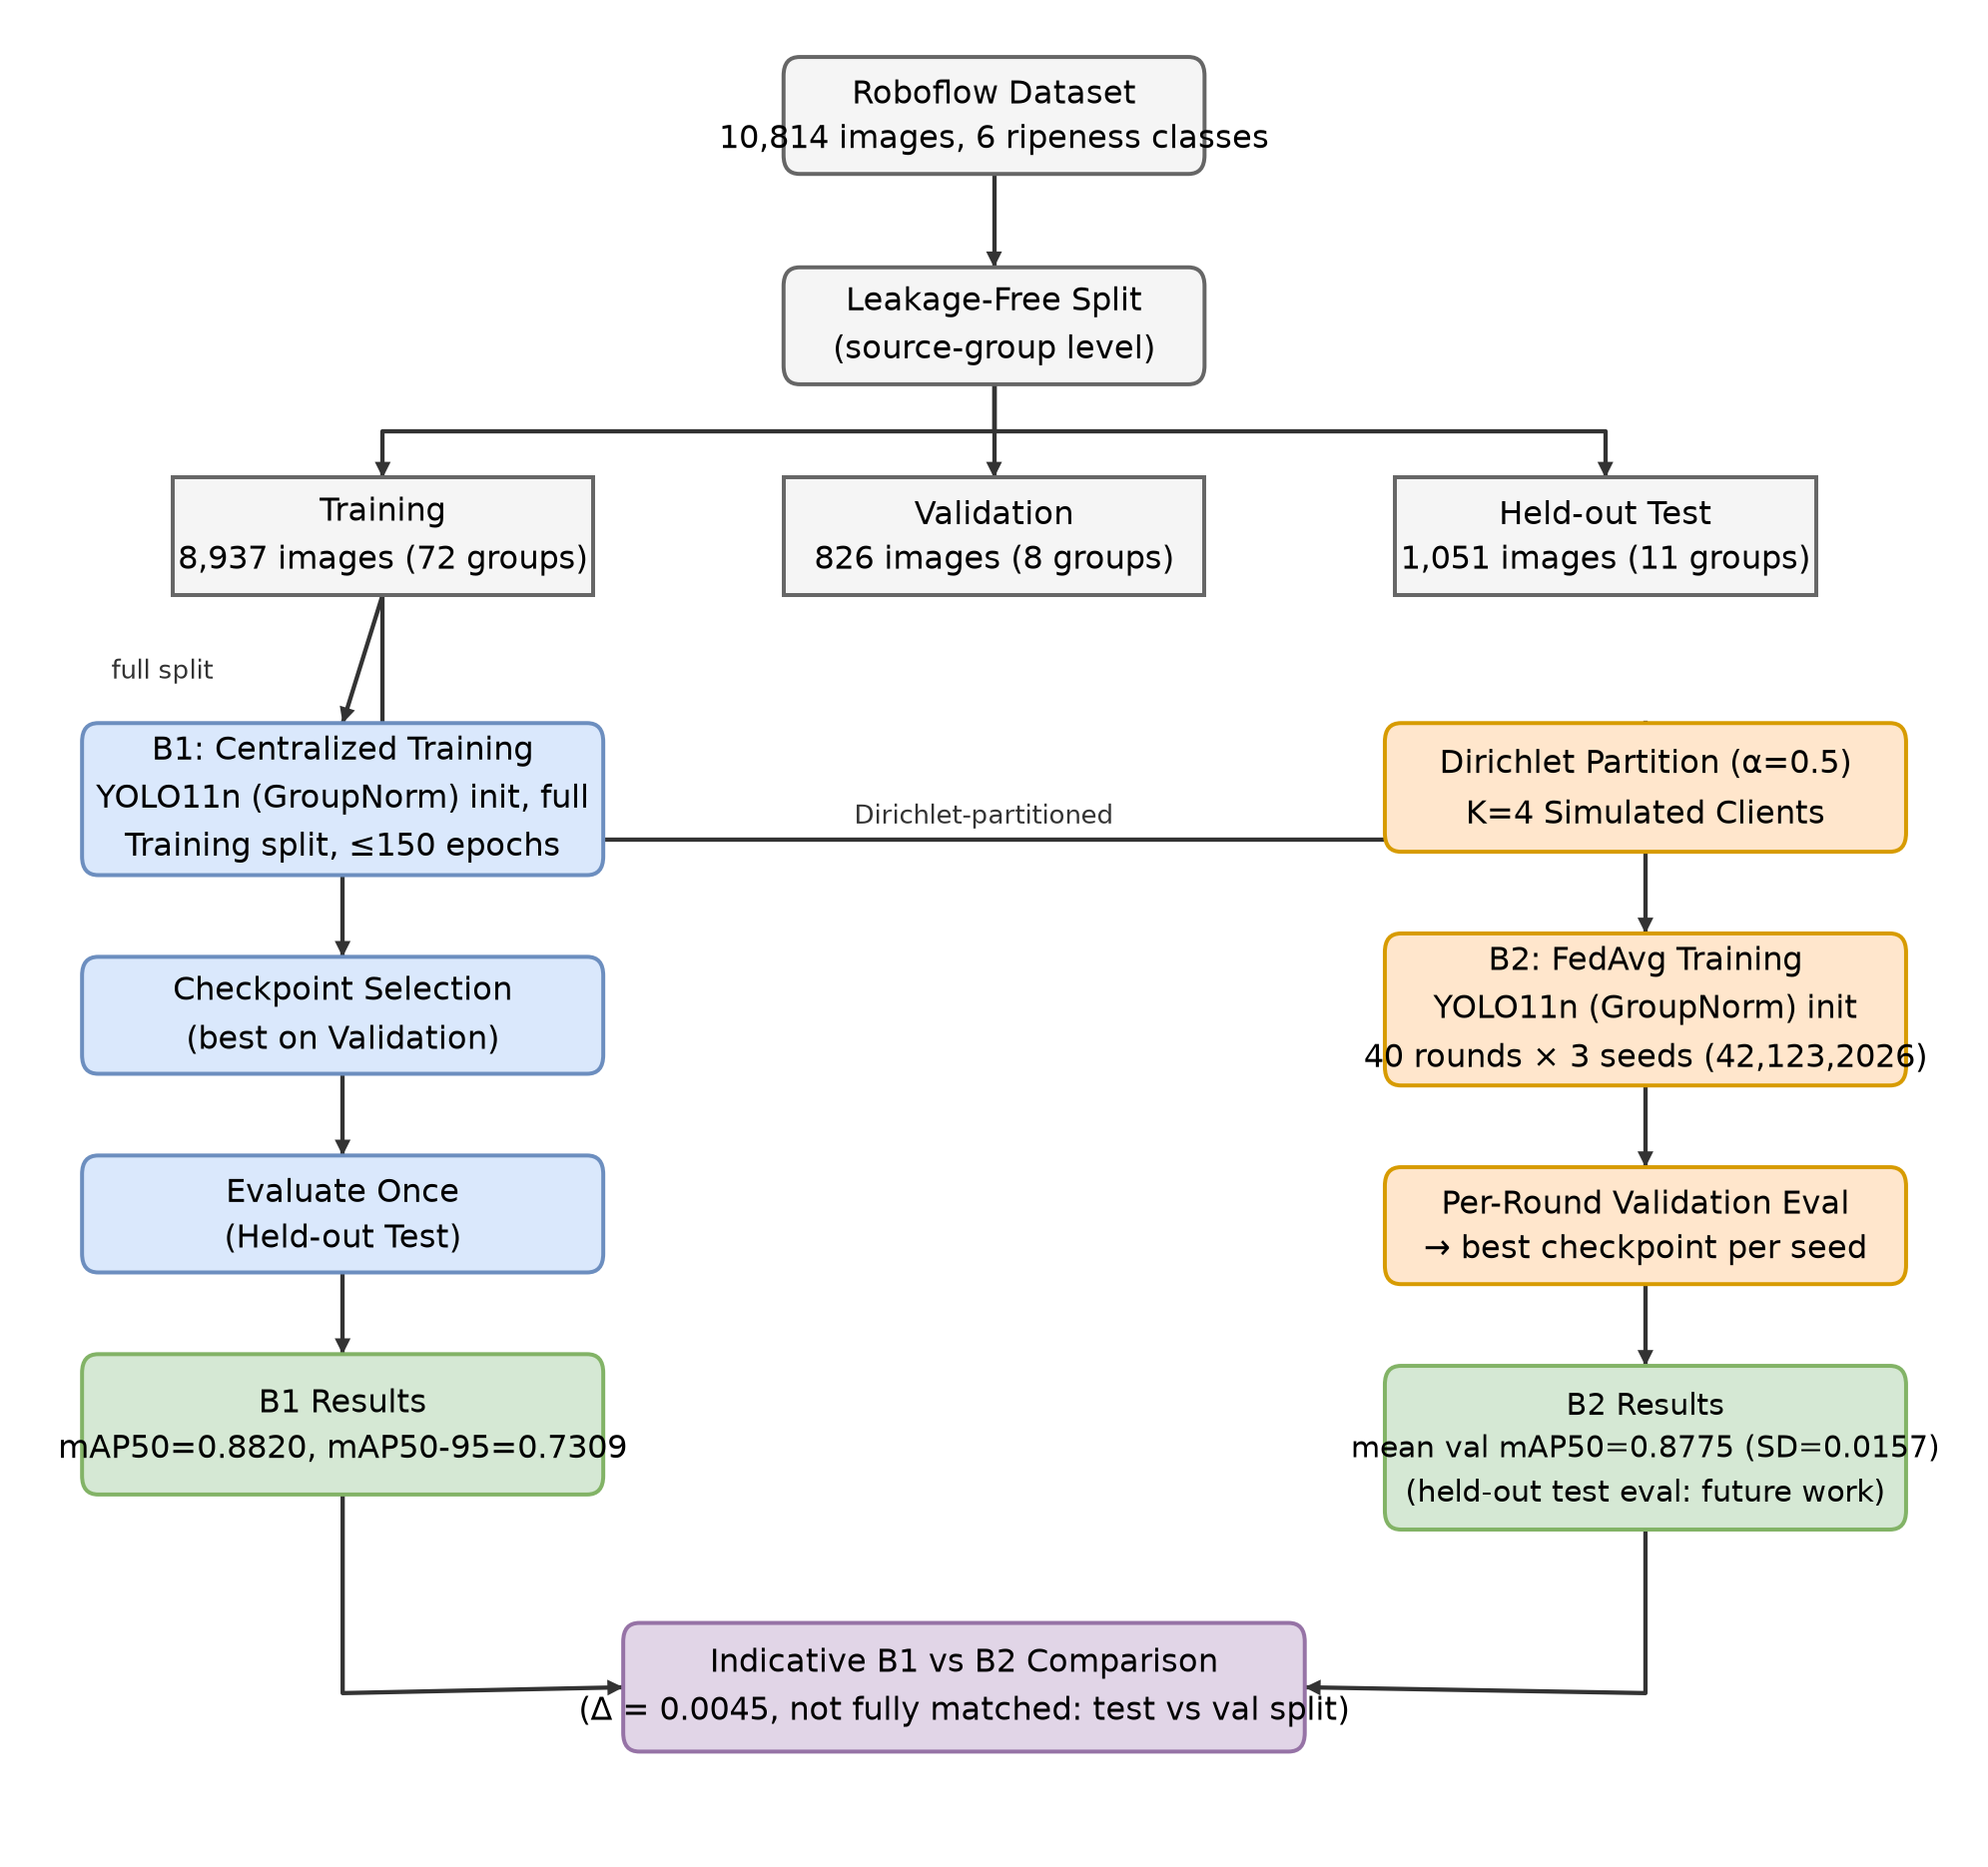
\includegraphics[width=0.95\linewidth]{figure1_workflow.png}
  \caption{Overall research workflow, from dataset preparation through the centralized (B1) reference path and the Non-IID federated (B2) multi-seed training path. B1 terminates as a single reference point; B2 feeds into the multi-seed reproducibility analysis reported in \emph{Results}. The two paths are not merged into a single comparison.}
  \label{fig:workflow}
\end{figure}

\subsection{Dataset}
This study uses the Palm Fruit Ripeness Detection dataset (version 2) sourced from Roboflow, comprising 10,814 images annotated for six ripeness-related classes: Abnormal, Empty Bunch, Overripe, Ripe, Underripe, and Unripe, in a manner broadly consistent with other publicly documented efforts to build annotated FFB ripeness datasets for deep-learning-based grading \cite{suharjito2023dataset}. The six classes reflect an operational grading protocol rather than a strict physiological maturity scale. Unripe and Underripe capture fruit at progressively earlier stages of colour change with little to no loose fruit; Ripe and Overripe correspond to the harvest-optimal and post-optimal stages, distinguished mainly by the proportion of loose fruit and the extent of colour development; and Empty Bunch and Abnormal represent non-standard bunch conditions, respectively bunches with most fruit already detached and bunches whose shape, density, or development departs from the normal pattern, rather than points on the ripeness continuum. This class structure is relevant to interpreting the per-class results reported in \emph{B1: Centralized Reference Baseline Results} below, since Ripe and Overripe are visually contiguous with their neighboring stages, whereas Empty Bunch and Abnormal are visually more distinct outlier conditions. Figure~\ref{fig:classes} shows a representative example image for each of the six classes.

\begin{figure}[H]
  \centering
  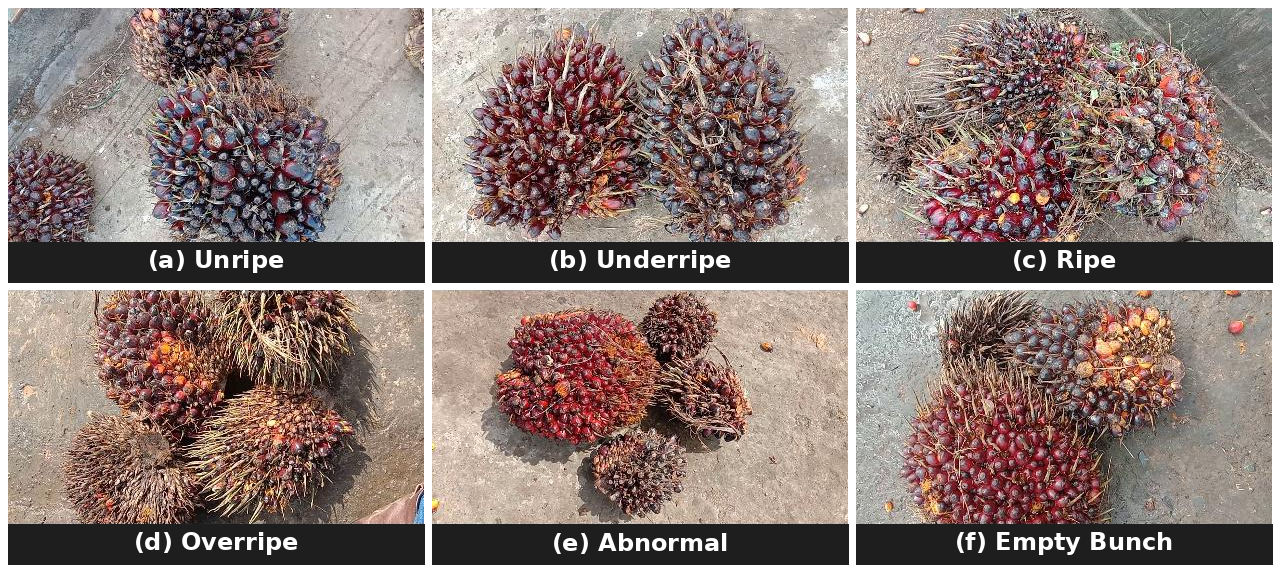
\includegraphics[width=0.95\linewidth]{figure2_sixclass_grid.png}
  \caption{Representative example images for each of the six ripeness-related classes (Abnormal, Empty Bunch, Overripe, Ripe, Underripe, Unripe).}
  \label{fig:classes}
\end{figure}

\subsection{Leakage-Free Split}
Images are grouped by their originating source group prior to splitting, and the train/validation/held-out-test partition is constructed at the source-group level to prevent source-related leakage across splits. The resulting split is summarized in Table~\ref{tab:split}. A leakage audit was performed to confirm: no source-group overlap between the training, validation, and test splits; no identical cross-split duplicate images; and no confirmed cross-split duplicate overlap according to the implemented audit procedure.

\begin{table}[H]
  \centering
  \caption{Leakage-free dataset split}
  \label{tab:split}
  \begin{tabular}{lrr}
    \toprule
    Split & Images & Source groups \\
    \midrule
    Training      & 8,937 & 72 \\
    Validation    & 826   & 8  \\
    Held-out test & 1,051 & 11 \\
    \bottomrule
  \end{tabular}
\end{table}

\subsection{Federated Partition}
Only the training subset (8,937 images) is partitioned among federated clients; the validation and held-out test splits are not partitioned. The federation uses K=4 clients under a Non-IID partition generated with a Dirichlet distribution ($\alpha = 0.5$, partition seed = 42). The Dirichlet distribution is a standard mechanism for constructing controllable Non-IID splits in federated learning research, since its concentration parameter directly governs the degree of class-distribution skew across clients without requiring additional heuristic allocation rules \cite{kairouz2021}. Table~\ref{tab:clients} and Figure~\ref{fig:client-dist} report the resulting client-level image distribution. The clients are simulated sample-level data shards and do not represent four physical plantations, estates, organizations, or devices; training is simulated sequentially on a single GPU. Images originating from one source group inside the training subset may be distributed across different clients; this does not violate the leakage-free train/validation/test split, since all client partitions are drawn exclusively from the training subset.

\begin{table}[H]
  \centering
  \caption{Federated client image distribution (K=4, Dirichlet $\alpha=0.5$, seed=42)}
  \label{tab:clients}
  \begin{tabular}{lrr}
    \toprule
    Client & Images & Share (\%) \\
    \midrule
    Client 0 & 860   & 9.62  \\
    Client 1 & 775   & 8.67  \\
    Client 2 & 5,305 & 59.36 \\
    Client 3 & 1,997 & 22.35 \\
    \midrule
    \textbf{Total} & \textbf{8,937} & \textbf{100.00} \\
    \bottomrule
  \end{tabular}
\end{table}

\begin{figure}[H]
  \centering
  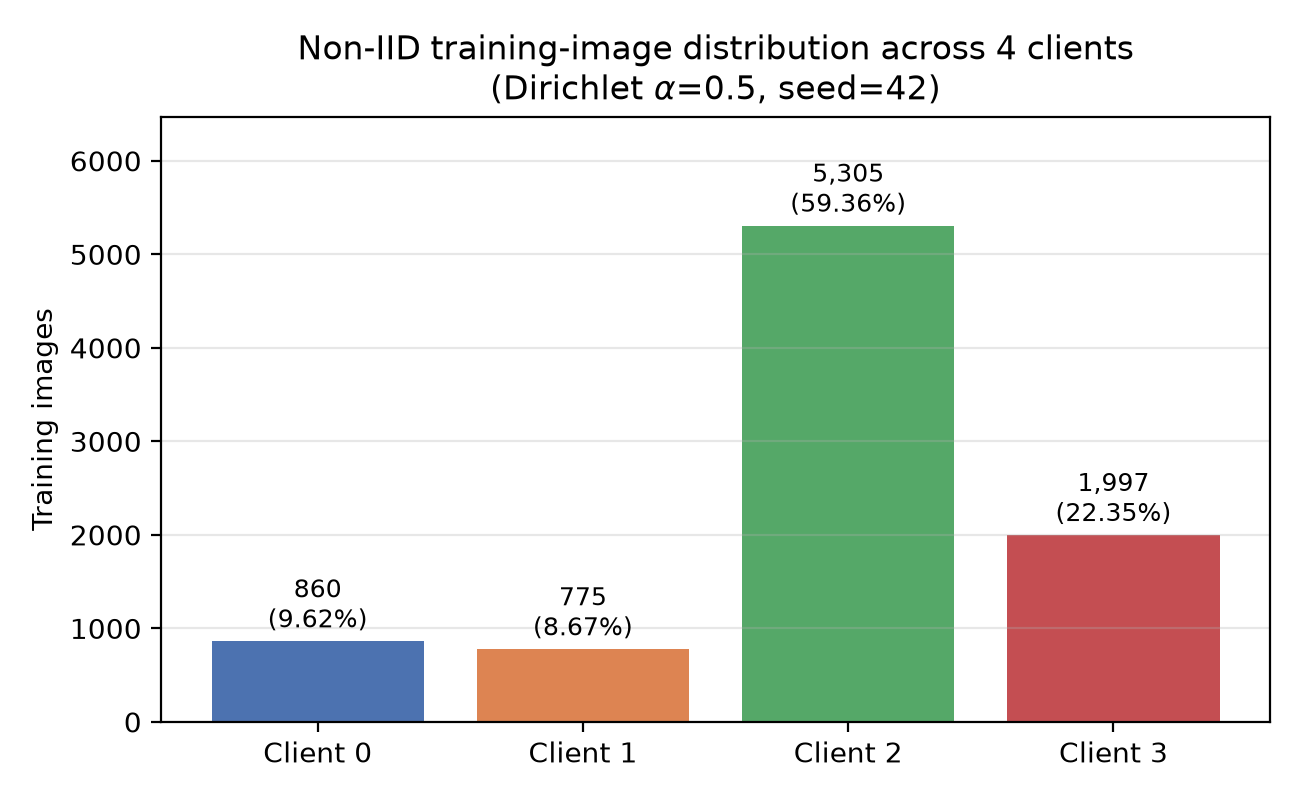
\includegraphics[width=0.7\linewidth]{figure_client_distribution.png}
  \caption{Non-IID training-image distribution across the four simulated federated clients (Dirichlet $\alpha=0.5$, seed 42).}
  \label{fig:client-dist}
\end{figure}

\subsection{Client Heterogeneity Measurement}
Table~\ref{tab:clients} quantifies client heterogeneity by training-image count. As a scalar summary of this quantity imbalance, the coefficient of variation across the four clients' image counts $\{860, 775, 5305, 1997\}$ (mean $\bar{n}=2234.25$) is computed using the population standard deviation, since these four clients constitute the entire population of clients in this experiment rather than a sample: $CV = \sqrt{\frac{1}{K}\sum_{k=1}^{K}(n_k-\bar{n})^2} \big/ \bar{n} \approx 0.822$, indicating substantial dispersion relative to the mean client size. This quantity measurement does not by itself establish class-distribution skew across clients, since a client could hold few images while still preserving the global class proportions.

Table~\ref{tab:client-class} reports the per-client, per-class bounding-box instance counts from the partition manifest, and Figure~\ref{fig:client-class} shows the corresponding per-client class proportions. For each client, class-level heterogeneity is summarized by the normalized Shannon entropy $H(c) = -\sum_{k=1}^{6} p_{c,k}\log p_{c,k} \big/ \log 6$ (1 = perfectly uniform across classes) and by the Jensen--Shannon divergence \cite{lin1991jsd} from the global (all-client-pooled) class distribution. Class-level and quantity-level heterogeneity are not aligned in this partition: Client 2, the largest client by image count (59.36\% share), has the \emph{lowest} divergence from the global class distribution (JSD = 0.0098, $H$ = 0.9238), whereas Client 1, the smallest client (8.67\% share), has the \emph{highest} divergence (JSD = 0.0422, $H$ = 0.8427), driven by its comparatively narrow concentration in Ripe and Underripe (33\% and 30\% of its instances) and near-absence of Empty Bunch and Overripe (1.8\% and 4.6\%). This means Client 2's large sample-weighted influence under FedAvg aggregation (\emph{Discussion}) is not, in this partition, also an influence toward a class-skewed signal; conversely, Client 1's small aggregation weight limits the practical impact of its comparatively skewed class composition.

\begin{table}[H]
  \centering
  \caption{Per-client, per-class training-instance (bounding-box) counts and heterogeneity statistics}
  \label{tab:client-class}
  \begin{tabular}{lrrrrrrrrr}
    \toprule
    Client & Abnormal & Empty Bunch & Overripe & Ripe & Underripe & Unripe & Total & $H(c)$ & JSD \\
    \midrule
    0 & 599  & 246 & 246  & 719  & 285  & 800  & 2,895  & 0.9346 & 0.0225 \\
    1 & 434  & 48  & 121  & 800  & 878  & 357  & 2,638  & 0.8427 & 0.0422 \\
    2 & 3,363 & 336 & 3,915 & 2,405 & 3,999 & 4,109 & 18,127 & 0.9238 & 0.0098 \\
    3 & 1,326 & 727 & 1,203 & 2,610 & 414  & 748  & 7,028  & 0.9067 & 0.0402 \\
    \bottomrule
  \end{tabular}
\end{table}

\begin{figure}[H]
  \centering
  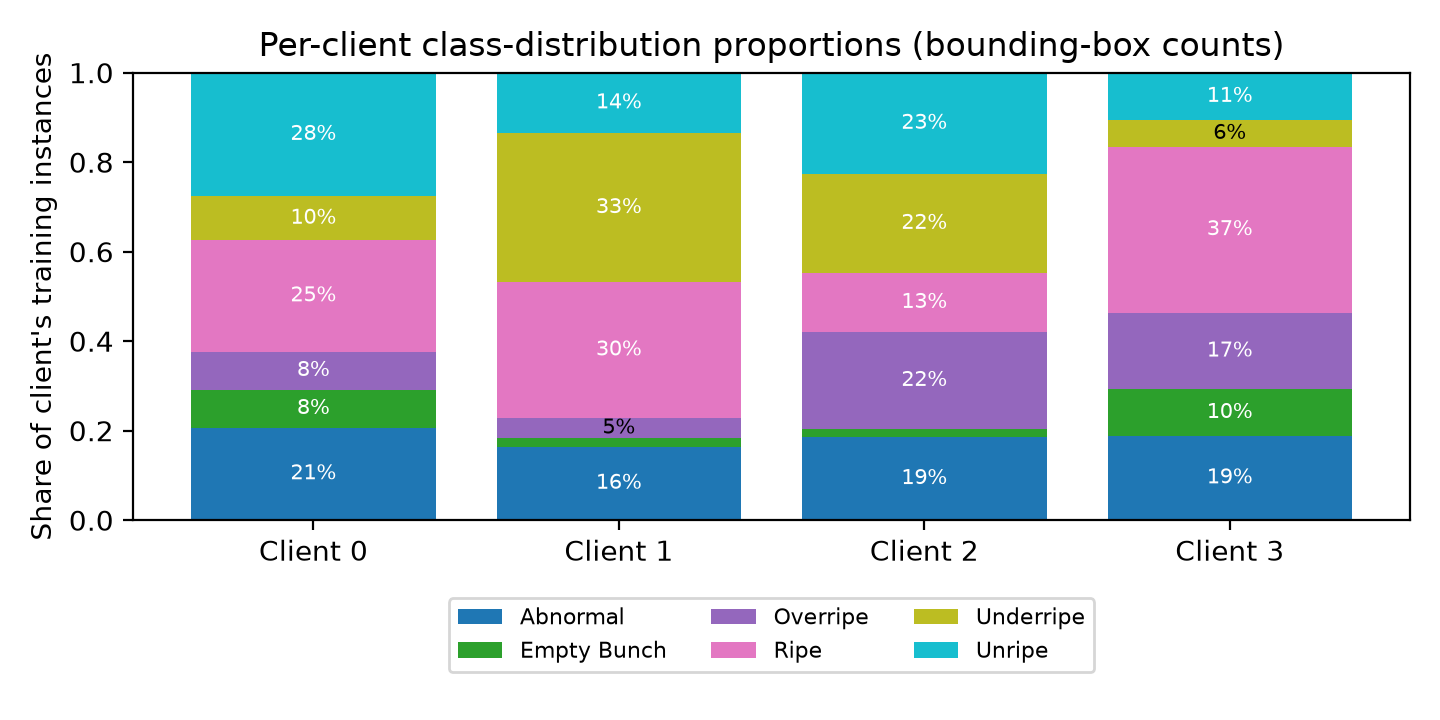
\includegraphics[width=0.85\linewidth]{figure_client_class_distribution.png}
  \caption{Per-client class-distribution proportions (bounding-box counts). Client 1, the smallest client by image count, shows the most concentrated class composition (Ripe + Underripe = 63\% of its instances); Client 2, the largest client, most closely tracks the global class distribution.}
  \label{fig:client-class}
\end{figure}

\subsection{Key Terminology}
To avoid ambiguity in the multi-seed protocol described below, this study distinguishes: the \emph{partition seed}, which controls the Dirichlet client-partition assignment and is fixed at 42 for all runs so that all three training seeds share an identical client data allocation; the \emph{training seed}, which controls stochastic elements of the training process itself (data shuffling order and augmentation sampling) and is varied across 42, 123, and 2026; a \emph{communication round}, one complete cycle of local training at all four clients followed by FedAvg aggregation (40 total per seed); a \emph{local epoch}, one full pass over a single client's local training partition within one communication round (2 per round); the \emph{best-validation checkpoint}, the model state saved after the communication round with the highest validation mAP50 for that seed; and the \emph{final-round checkpoint}, the model state after the last (40th) communication round, regardless of whether it is also the best-validation checkpoint.

\subsection{Model Architecture}
The base detector is YOLO11n \cite{jocher2024}, initialized from weights pretrained on the COCO dataset \cite{lin2014coco}, with an input resolution of $960\times960$. The adjusted model contains 2,591,010 parameters. All Batch Normalization layers were converted to Group Normalization \cite{wu2018groupnorm}, since cross-sample batch statistics are known to become unreliable under small, Non-IID per-client batches in federated settings \cite{li2021fedbn}; a final architecture audit confirmed 0 remaining BatchNorm modules and 81 GroupNorm modules across the network. This substitution is applied consistently across B1 and B2 so that normalization type is not a confounding factor when interpreting results, and is reported here strictly as a design choice, not as an empirically demonstrated performance or stability improvement, since no BatchNorm-versus-GroupNorm ablation was run in this study (see \emph{Limitations}). A fixed convolution inside the Distribution Focal Loss (DFL) module is set with \texttt{requires\_grad=False} and is excluded from optimization.

\subsection{Implementation Environment}
All training and evaluation was performed on a single workstation equipped with an NVIDIA GeForce RTX 4080 GPU (16 GB VRAM), a multi-core CPU, and 32 GB of system RAM. The implementation used Python 3.10, PyTorch 2.5.1 with CUDA 12.1, and Ultralytics 8.4.51 for the YOLO11 model definition and training loop. Federated simulation (B2) executed clients sequentially on this single GPU within each communication round, rather than concurrently across separate physical machines; this is consistent with the simulated, single-host framing of the federation described in the \emph{Federated Partition} subsection above.

\subsection{B1: Centralized Reference Baseline}
B1 is a centralized reference baseline (not a mathematical upper bound), trained for a maximum of 150 epochs with an early-stopping patience of 30 epochs, batch size 16, and input size $960\times960$. B1 is trained on the full training subset (8,937 images) in a single, non-federated run, using the same underlying training images that are subsequently partitioned across the four clients in B2; this ensures that any performance difference between B1 and B2 reflects the effect of federation and data partitioning rather than a difference in the underlying training data pool. The reported checkpoint is selected using validation performance and subsequently evaluated once on the held-out test split.

\subsection{B2: Non-IID Federated Training Protocol (FedAvg)}
B2 applies FedAvg \cite{mcmahan2017fedavg,konecny2016} under the same K=4, Dirichlet $\alpha=0.5$, partition-seed-42 configuration described above, using 40 communication rounds, 2 local epochs per round, SGD optimization (learning rate 0.01, momentum 0.9, weight decay 0.0005), batch size 8, input size 960, and no warmup. Training was repeated with three training seeds (42, 123, 2026, per the \emph{Key Terminology} subsection above) that vary only the stochastic training realization and were not selected for any special numerical property; the partition seed remains fixed at 42 across all three runs. This replication is the basis for the reproducibility analysis reported in \emph{Results} below.

\subsection{Held-Out Test Protocol}
The held-out test split is reserved strictly for final reporting and is not used to choose hyperparameters, communication rounds, or checkpoints. B1 was evaluated on the held-out test split only after its checkpoint was locked, and this result was not used to choose or modify the configuration of B2. For B2, each of the three locked seed checkpoints is intended for eventual evaluation on the same held-out test split; at the time of writing, B2 results are reported on the validation split, and validation and held-out test metrics are not mixed in direct comparisons within this manuscript.

\subsection{Evaluation Metrics}
Detection performance is reported using standard object-detection metrics: mAP50, mAP50-95, precision, and recall, computed on the split specified in each results table (the held-out test split for B1; the validation split for B2).

\subsection{Reproducibility}
Partition seed 42 is used for the federated partitioning underlying B2. B2 is repeated using three training seeds (42, 123, 2026) that vary only the stochastic training realization; the partition seed remains fixed across all three runs. Each seed configures Ultralytics' deterministic training mode (\texttt{deterministic=True}, applying \texttt{torch.manual\_seed}, NumPy and Python RNG seeding, and constrained cuDNN behavior); additionally, this implementation applies a targeted fix so that the per-round dataloader's shuffle order and worker augmentation seeds are re-seeded from the experiment seed rather than a library-internal constant, since this was found to be otherwise unaffected by \texttt{args.seed} in the underlying framework version used. Under this configuration, varying only the training seed while holding partition, initialization, and optimizer configuration fixed is expected to alter data shuffling order and augmentation sampling from the first training step onward, which is the intended source of the stochastic variation characterized in this study. Implementation code, dataset-splitting manifests, and configuration files are available from the corresponding author upon reasonable request.

\section{Results}

This section reports results for the centralized reference baseline (B1) and the multi-seed Non-IID federated training protocol (B2), organized to separate outcome-level reproducibility (peak validation performance across seeds) from trajectory-level reproducibility (convergence behavior across communication rounds).

\subsection{Centralized Reference Performance}
Table~\ref{tab:b1} reports the finalized held-out test results for B1.

\begin{table}[H]
  \centering
  \caption{B1 centralized reference baseline --- held-out test results}
  \label{tab:b1}
  \begin{tabular}{lrr}
    \toprule
    Class & AP50 & AP50-95 \\
    \midrule
    Abnormal     & 0.9924 & 0.8462 \\
    Empty Bunch  & 0.9817 & 0.7521 \\
    Overripe     & 0.9406 & 0.6968 \\
    Ripe         & 0.5571 & 0.4757 \\
    Underripe    & 0.8275 & 0.7382 \\
    Unripe       & 0.9929 & 0.8766 \\
    \midrule
    \textbf{Overall mAP} & \textbf{0.8820} & \textbf{0.7309} \\
    \bottomrule
  \end{tabular}
\end{table}

Overall Precision = 0.8745; Overall Recall = 0.8653. Ripe is currently the weakest-performing class in B1 by both AP50 and AP50-95. The normalized confusion matrix (Figure~\ref{fig:b1-ap50}) identifies the specific cause: of true Ripe instances, only 60\% are predicted as Ripe, while 35\% are misclassified as Underripe and 5\% as Overripe -- i.e., the model's errors on Ripe are concentrated almost entirely on its two adjacent ripeness stages, not on visually unrelated classes. Consistent with the class structure described in the \emph{Dataset} subsection above, the two structurally distinct classes (Abnormal, Empty Bunch) and the least visually ambiguous ripeness stage (Unripe) achieve the highest AP50 values (all $\ge 0.9817$), while Ripe, a mid-sequence stage bordered by both Underripe and Overripe, achieves the lowest AP50 (0.5571). Underripe (0.8275), also a mid-sequence stage, shows an intermediate AP50 value broadly consistent with this pattern, and is itself confused with Ripe in 35\% of its true instances (a symmetric, bidirectional Ripe/Underripe boundary error), while Overripe (0.9406) is confused with Ripe in only 5\% of its true instances, explaining why it does not fit the pattern as closely. Figure~\ref{fig:b1-ap50} presents the confusion matrix and precision-recall curve underlying Table~\ref{tab:b1} for visual inspection, and Figure~\ref{fig:b1-qual} provides qualitative detection examples, including at least one from the weaker-performing Ripe class.

\begin{figure}[H]
  \centering
  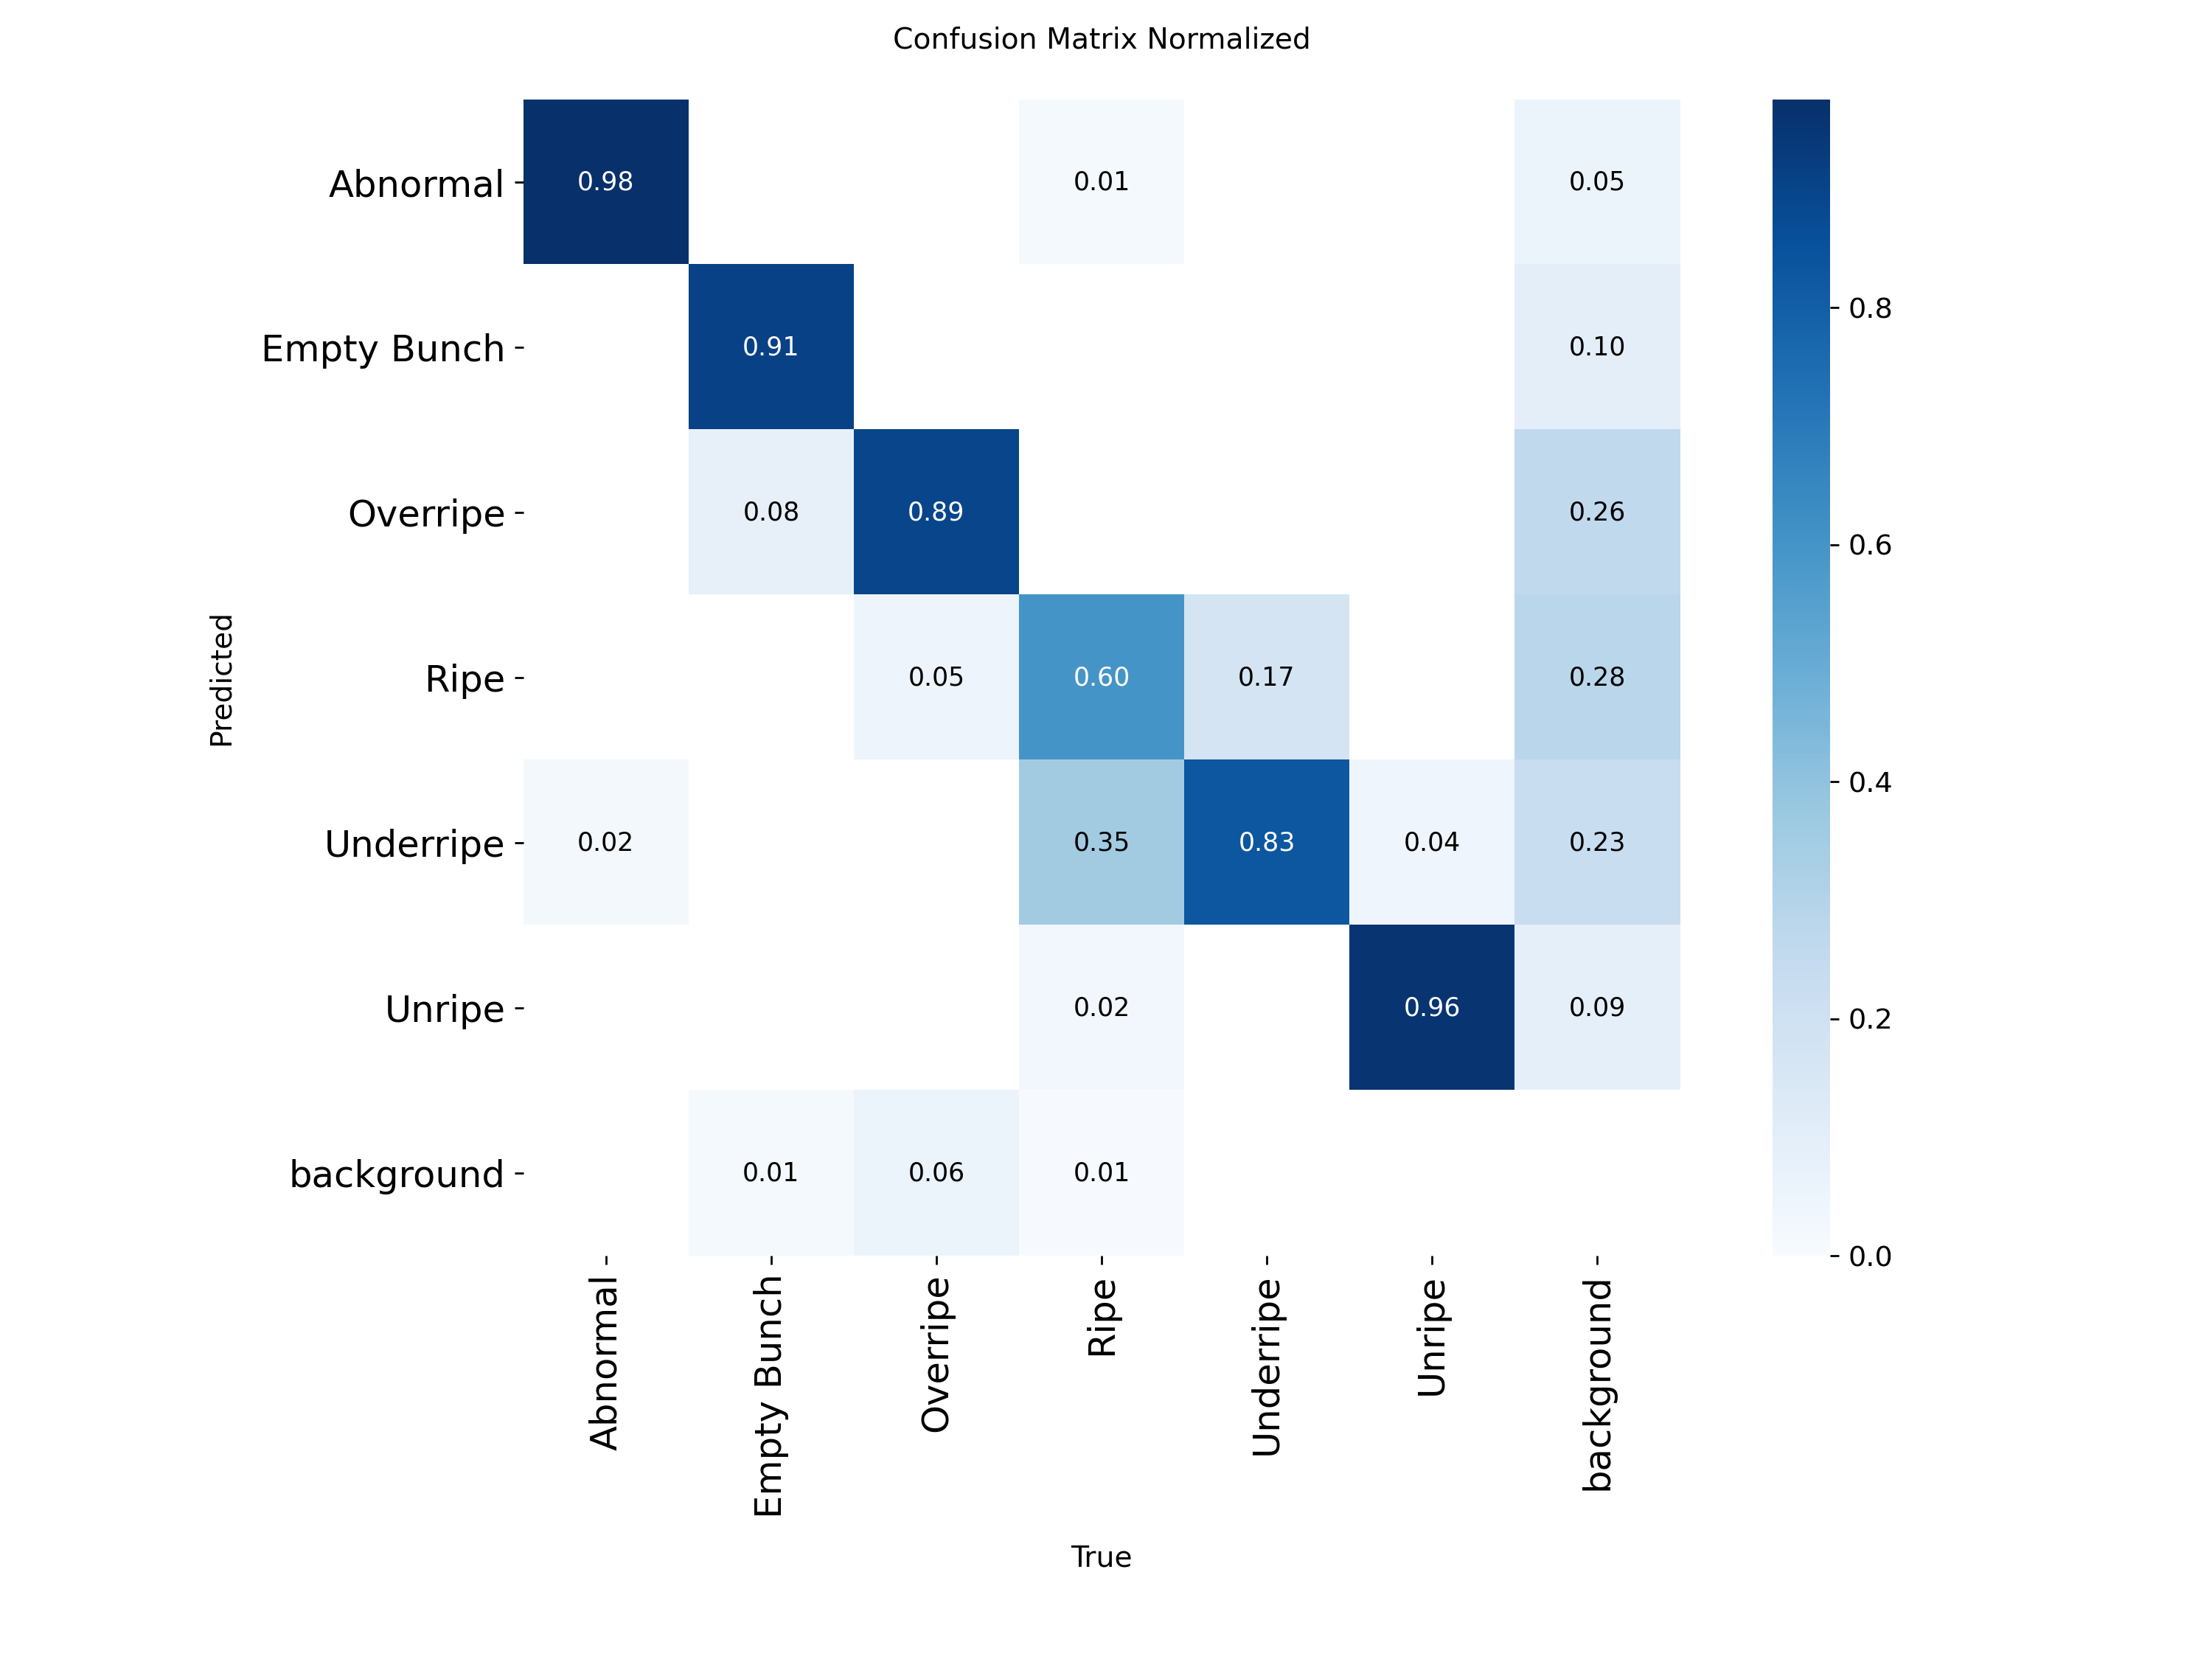
\includegraphics[width=0.75\linewidth]{confusion_matrix_normalized.png}
  \caption{B1 (centralized) normalized confusion matrix on the held-out test split. Rows are predicted classes, columns are true classes; values are row-normalized fractions (real Ultralytics evaluation output from \texttt{scripts/42\_generate\_b1\_test\_plots.py}, matches Table~\ref{tab:b1} exactly).}
  \label{fig:b1-ap50}
\end{figure}

\begin{figure}[H]
  \centering
  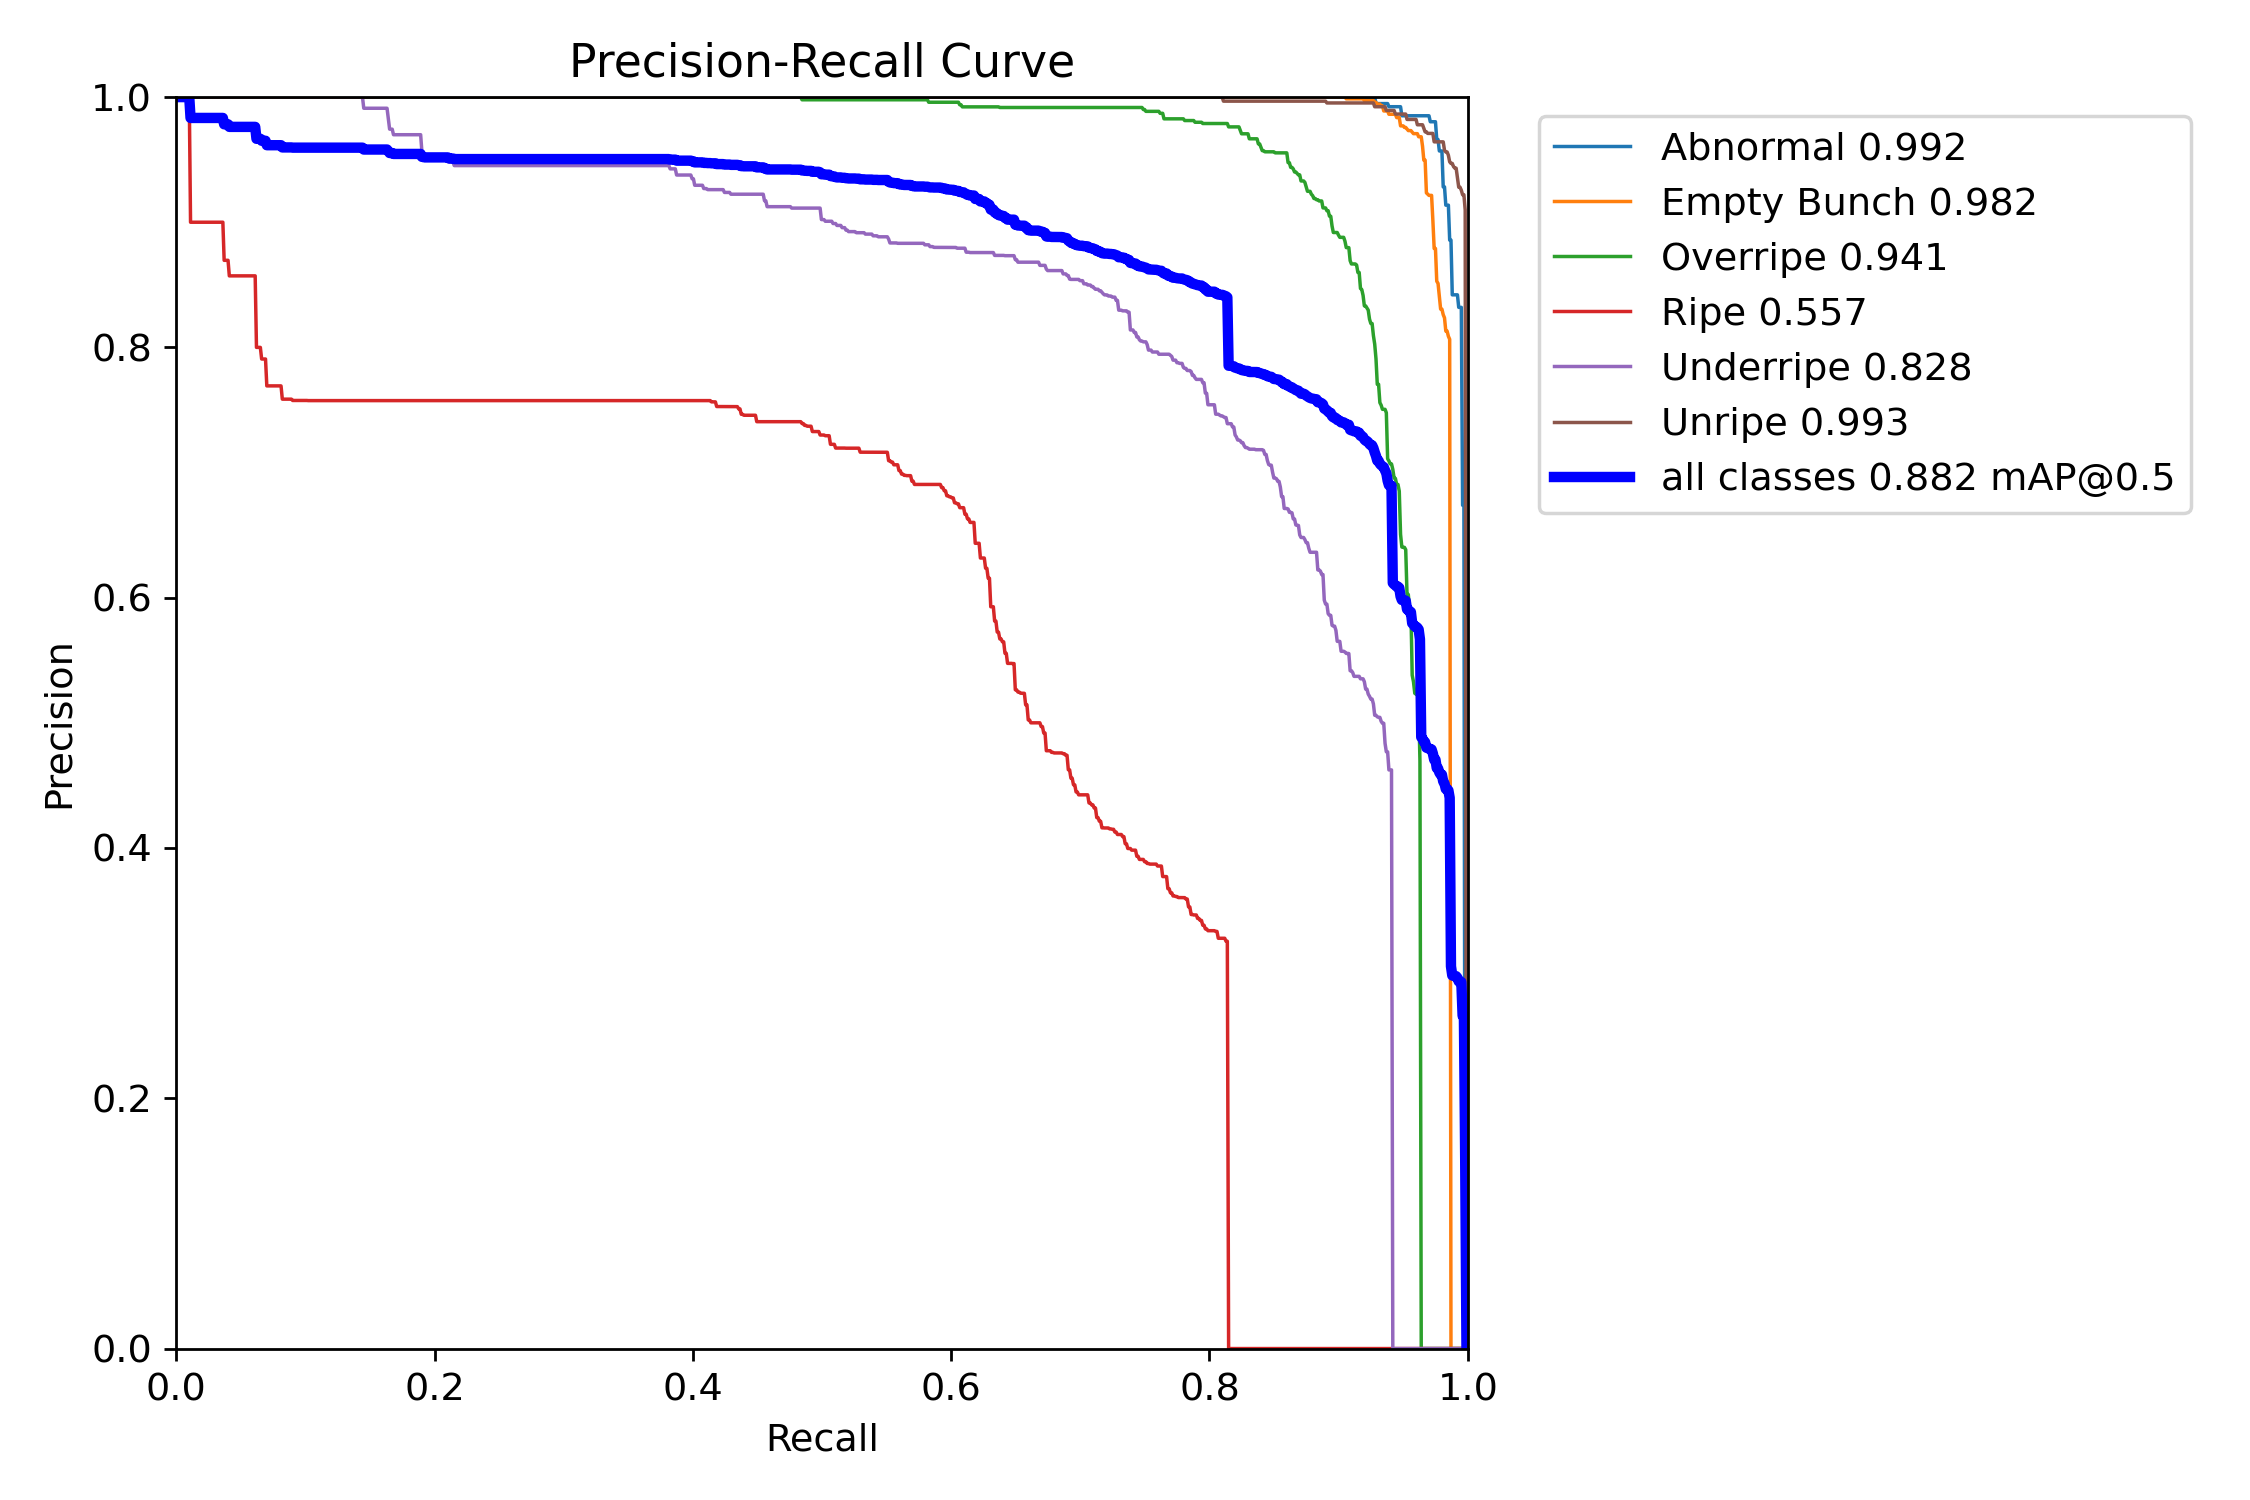
\includegraphics[width=0.75\linewidth]{box_PR_curve.png}
  \caption{B1 (centralized) precision-recall curve on the held-out test split, per class and overall (mAP@0.5 = 0.882, matching Table~\ref{tab:b1}).}
  \label{fig:b1-pr}
\end{figure}

\begin{figure}[H]
  \centering
  \begin{minipage}{0.48\linewidth}
    \centering
    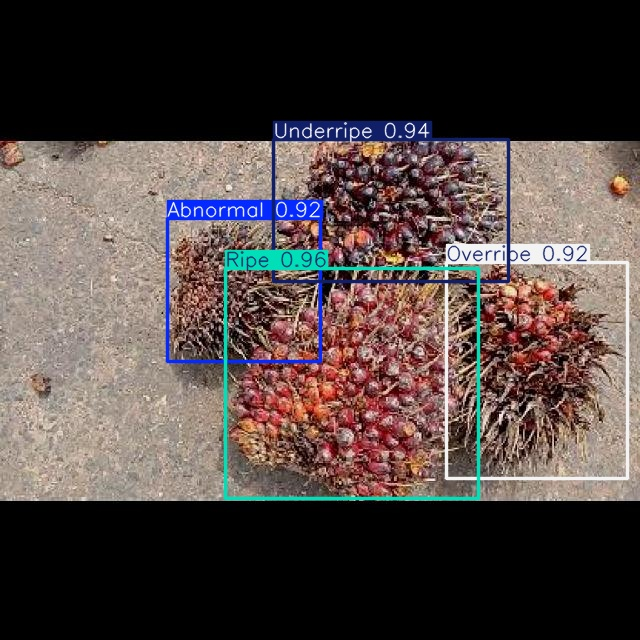
\includegraphics[width=\linewidth]{qual_ripe.jpg}\\
    \small (a) Ripe (conf.\ 0.96)
  \end{minipage}\hfill
  \begin{minipage}{0.48\linewidth}
    \centering
    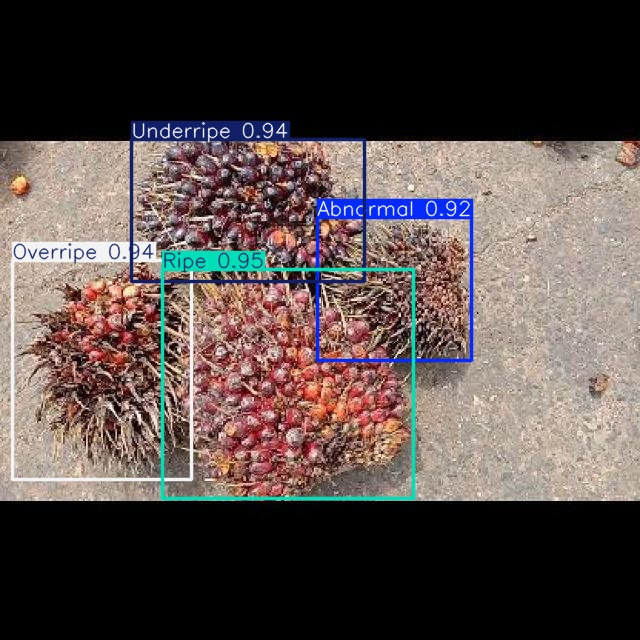
\includegraphics[width=\linewidth]{qual_abnormal.jpg}\\
    \small (b) Abnormal (conf.\ 0.92)
  \end{minipage}

  \vspace{0.5em}
  \begin{minipage}{0.48\linewidth}
    \centering
    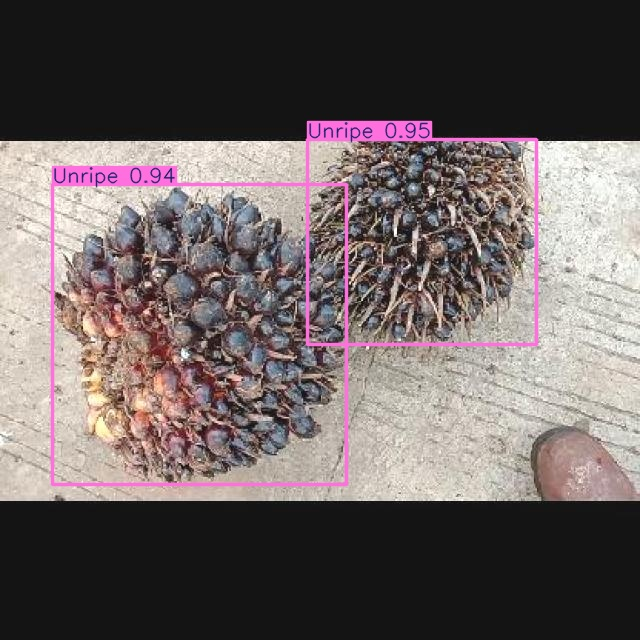
\includegraphics[width=\linewidth]{qual_unripe.jpg}\\
    \small (c) Unripe (conf.\ 0.94--0.95)
  \end{minipage}\hfill
  \begin{minipage}{0.48\linewidth}
    \centering
    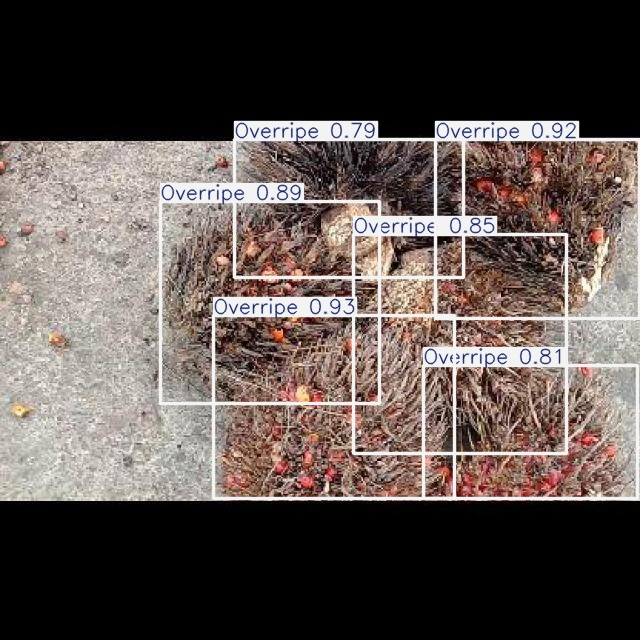
\includegraphics[width=\linewidth]{qual_overripe.jpg}\\
    \small (d) Overripe (conf.\ 0.79--0.93)
  \end{minipage}
  \caption{Qualitative detection examples from B1 on held-out test images -- real \texttt{model.predict()} output with predicted bounding boxes, class labels, and confidence scores (generated by \texttt{scripts/53\_generate\_b1\_qualitative\_examples.py}, GT-label-driven selection, one distinct image per class). (a) and (b) are two augmented crops of the same held-out multi-bunch scene (Underripe, Abnormal, Ripe, and Overripe bunches co-occurring in one frame); they are shown together because Ripe -- B1's weakest-performing class -- is correctly detected at high confidence (0.96) in (a). (c) and (d) show distinct scenes for the Unripe and Overripe classes.}
  \label{fig:b1-qual}
\end{figure}

\subsection{Multi-Seed Federated Validation Performance}
Table~\ref{tab:b2} reports B2 validation results across the three training seeds. These are validation-set results; a direct B1-vs-B2 performance gap is not computed here, since B1 is reported on the held-out test split while B2 is reported on validation. No comparison against B1 is drawn in this subsection; see \emph{Held-Out-Test Evaluation Protocol} below for the genuinely matched held-out-test comparison.

\begin{table}[H]
  \centering
  \caption{B2 (FedAvg) --- three-seed validation results}
  \label{tab:b2}
  \begin{tabular}{lrrrl}
    \toprule
    Seed & Best round & mAP50 & mAP50-95 & Prec.\ / Rec. \\
    \midrule
    42   & 9  & 0.8850 & 0.7431 & 0.8717 / 0.8616 \\
    123  & 11 & 0.8594 & 0.7145 & 0.8139 / 0.8422 \\
    2026 & 40 & 0.8880 & 0.7544 & 0.8868 / 0.9104 \\
    \midrule
    \textbf{Mean} & --- & \textbf{0.8775} & \textbf{0.7374} & 0.8574 / 0.8714 \\
    \textbf{SD}   & --- & \textbf{0.0157} & \textbf{0.0206} & 0.0385 / 0.0352 \\
    \bottomrule
  \end{tabular}
\end{table}

This outcome-level result -- a small SD (0.0157) of validation mAP50 across three independent training seeds -- is the primary reproducibility evidence reported in this study: it indicates that the federated configuration converges to a comparable operating point regardless of the stochastic training realization.

\subsection{Convergence Trajectory Across Seeds}
Figure~\ref{fig:b2-convergence} presents the per-round validation mAP50 trajectory for the three seeds and is the primary evidence for the trajectory-level component of this study's reproducibility claim. The best-validation checkpoint round varied substantially across seeds: round 9 for seed 42, round 11 for seed 123, and round 40 (the final round) for seed 2026 -- an approximately four-fold spread. This indicates that, although peak validation performance is comparable across all three seeds (best-checkpoint mAP50 range: 0.8594--0.8880), convergence \emph{speed} under this Non-IID partition is sensitive to the stochastic training trajectory: outcome-level reproducibility does not imply trajectory-level reproducibility. Note that ``peak'' here refers specifically to each seed's best-validation checkpoint (Table~\ref{tab:b2}); round-40 (final) values for seeds 42 and 123 are reported and discussed in \emph{Best-Round versus Final-Round Behavior} below (Table~\ref{tab:best-final}), which shows a mild post-peak decline for both seeds rather than sustained or recovered performance.

\begin{figure}[H]
  \centering
  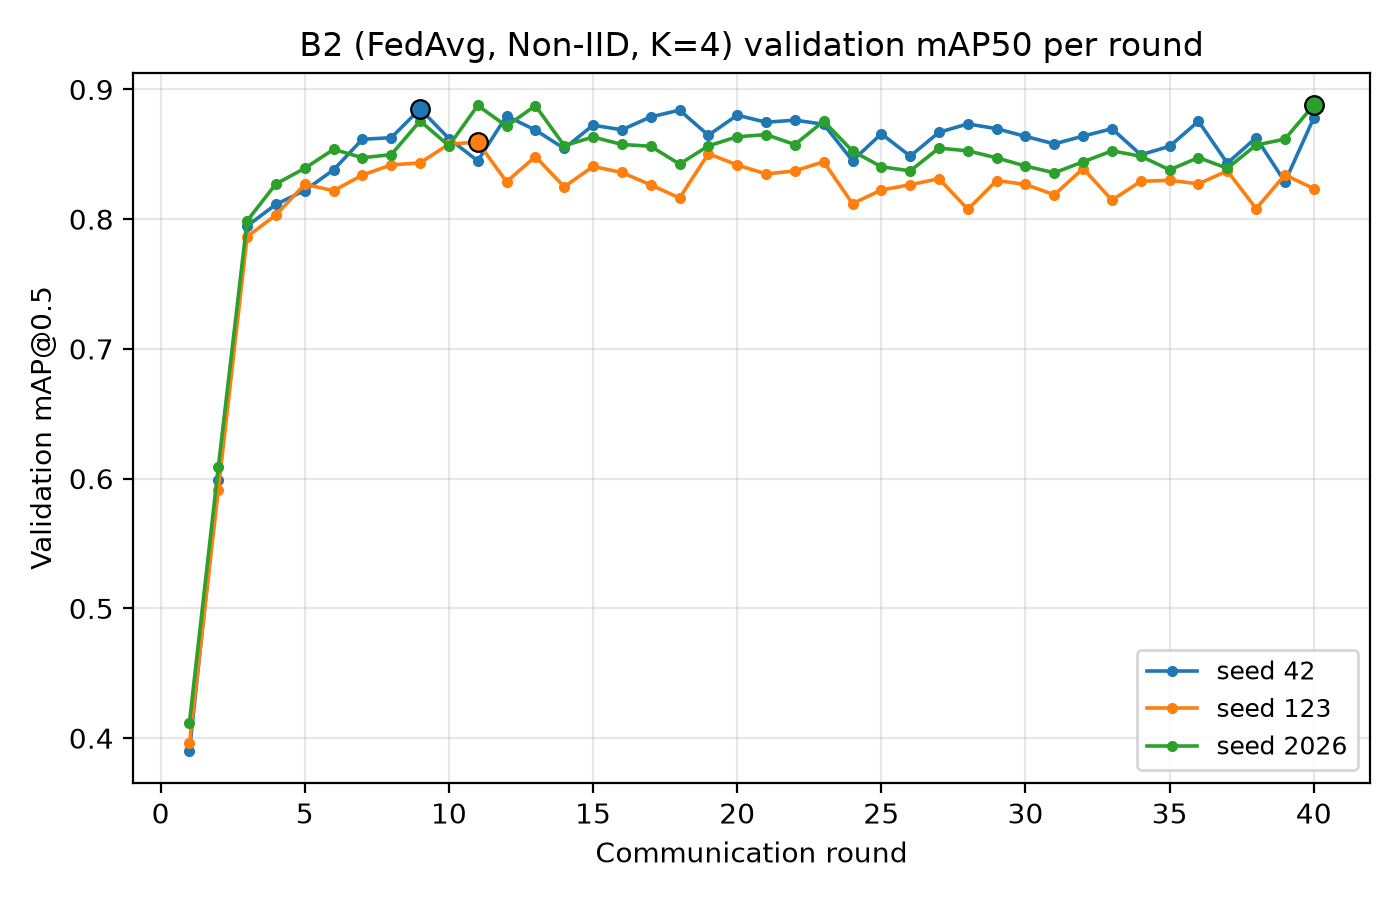
\includegraphics[width=0.85\linewidth]{figure_b2_convergence.png}
  \caption{B2 (FedAvg, Non-IID, K=4) validation mAP50 per communication round across three independent training seeds (42, 123, 2026). Filled markers denote each seed's best-validation round (Table~\ref{tab:b2}), illustrating substantial trajectory-level variance (round 9--40) despite comparable peak-validation performance.}
  \label{fig:b2-convergence}
\end{figure}

\subsection{Best-Round versus Final-Round Behavior}
Table~\ref{tab:best-final} compares each seed's best-validation checkpoint against its final-round (round 40) checkpoint, computed from the per-round validation history recorded during training. For seed 2026, the best and final rounds coincide by construction (best round = 40), so the difference is zero. For seeds 42 and 123, validation mAP50 at round 40 is lower than at the best round by 0.0070 and 0.0359 respectively, indicating that performance is not monotonically maintained after the peak for these two seeds -- a mild decline rather than catastrophic degradation, but one that would be invisible to a report using only each seed's best-checkpoint number.

\begin{table}[H]
  \centering
  \caption{Best-validation versus final-round (round 40) checkpoint performance}
  \label{tab:best-final}
  \begin{tabular}{lrrrr}
    \toprule
    Seed & Best round & Best mAP50 & Final (round 40) mAP50 & $\Delta$ (Best $-$ Final) \\
    \midrule
    42   & 9  & 0.8850 & 0.8780 & 0.0070 \\
    123  & 11 & 0.8594 & 0.8235 & 0.0359 \\
    2026 & 40 & 0.8880 & 0.8880 & 0.0000 \\
    \bottomrule
  \end{tabular}
\end{table}

\subsection{Per-Class Federated Stability}
Global mAP50 stability across seeds (Table~\ref{tab:b2}) does not by itself establish that every individual ripeness class is equally stable; a class with high inter-seed variance could be masked by a low-variance aggregate metric if its AP50 magnitude is small relative to others. Table~\ref{tab:per-class-stability} reports each seed's per-class AP50, taken at that seed's own best-validation checkpoint (Table~\ref{tab:b2}), computed from the corresponding validation history record for each seed. Per-class SD varies substantially across classes and is, for two classes, markedly larger than the global mAP50 SD of 0.0157: Underripe shows the highest inter-seed variance (SD = 0.0727, more than four times the global figure), followed by Unripe (SD = 0.0277), while Abnormal, Empty Bunch, and Overripe remain comparatively stable (SD $\le$ 0.0045--0.0140). This directly answers Supporting Research Question (iii): global mAP50 stability masks substantial per-class instability, concentrated in Underripe -- the same class family (mid-sequence ripeness stages with gradual visual transitions) already identified as B1's weakest class (\emph{B1: Centralized Reference Baseline Results}).

\begin{table}[H]
  \centering
  \caption{Per-class AP50 across the three B2 training seeds (each seed's own best-validation checkpoint)}
  \label{tab:per-class-stability}
  \begin{tabular}{lrrrrr}
    \toprule
    Class & Seed 42 & Seed 123 & Seed 2026 & Mean & SD \\
    \midrule
    Abnormal    & 0.9586 & 0.9670 & 0.9566 & 0.9607 & 0.0045 \\
    Empty Bunch & 0.9950 & 0.9858 & 0.9950 & 0.9919 & 0.0043 \\
    Overripe    & 0.9867 & 0.9836 & 0.9928 & 0.9877 & 0.0038 \\
    Ripe        & 0.9490 & 0.9598 & 0.9825 & 0.9638 & 0.0140 \\
    Underripe   & 0.5108 & 0.3866 & 0.5592 & 0.4855 & 0.0727 \\
    Unripe      & 0.9099 & 0.8735 & 0.8420 & 0.8751 & 0.0277 \\
    \bottomrule
  \end{tabular}
\end{table}

\subsection{Held-Out-Test Evaluation Protocol}
All three of B2's validation-selected seed checkpoints (locked before this evaluation, using the same held-out-test split and evaluation configuration as B1) were evaluated exactly once, yielding a genuinely matched centralized-versus-federated comparison. B2's three-seed mean held-out-test mAP50 is 0.8031 (SD = 0.0319), against B1's 0.8820 -- a gap of 0.0789. This gap is substantially larger than the 0.0045 gap suggested by the earlier indicative comparison (B1 held-out test versus B2 mean \emph{validation} mAP50, Section~\ref{sec:results}), because each of the three B2 seeds shows a non-trivial validation-to-test drop (0.8850$\to$0.7951 for seed 42, 0.8594$\to$0.7760 for seed 123, 0.8880$\to$0.8383 for seed 2026) that the validation-only comparison could not capture. The held-out-test spread across seeds (SD = 0.0319) is also roughly twice the validation-split spread (SD = 0.0157), indicating that cross-seed variability itself is larger on held-out test than validation suggested.

\begin{table}[H]
  \centering
  \caption{Matched held-out-test comparison}
  \label{tab:matched}
  \begin{tabular}{llrr}
    \toprule
    Model & Split & mAP50 & mAP50-95 \\
    \midrule
    B1 (centralized) & Held-out test & 0.8820 & 0.7309 \\
    B2 seed 42       & Held-out test & 0.7951 & 0.6528 \\
    B2 seed 123      & Held-out test & 0.7760 & 0.6373 \\
    B2 seed 2026     & Held-out test & 0.8383 & 0.6859 \\
    B2 mean (SD)     & Held-out test & 0.8031 (0.0319) & 0.6587 (0.0246) \\
    \bottomrule
  \end{tabular}
\end{table}

\section{Discussion}

The multi-seed results reported here separate two distinct notions of federated-training reliability that are often conflated in single-run reports: \emph{outcome-level reproducibility} (how similar the final achievable performance is across independent runs) and \emph{trajectory-level reproducibility} (how similar the path -- specifically, the number of communication rounds -- taken to reach that performance is). B1's held-out test results are reported here as a single reference point (mAP50 = 0.8820, mAP50-95 = 0.7309), with Ripe currently the weakest-performing class by a wide margin (AP50 = 0.5571 versus 0.8275 or higher for all other classes); a definitive cause cannot be asserted without confusion-matrix or dataset-level analysis, but plausible contributing factors include gradual visual transitions into and out of the Ripe stage and possible visual overlap with the adjacent Underripe and Overripe classes, which future work should investigate directly.

\subsection*{Outcome-Level Reproducibility}
The three B2 seeds converge to a comparable peak validation mAP50 (0.8594--0.8880, SD = 0.0157), which is consistent with -- though not proof of -- FedAvg being a numerically stable aggregation procedure under this specific Non-IID partition (Dirichlet $\alpha=0.5$, K=4). This is the strongest reproducibility evidence in this study, since it is directly measured across three independent stochastic training realizations rather than inferred from a single run. However, the matched held-out-test evaluation of the same three checkpoints (Table~\ref{tab:matched}) shows a wider spread (0.7760--0.8383, SD = 0.0319) -- roughly twice the validation-split SD. Outcome-level reproducibility measured on validation alone therefore appears to understate the cross-seed variability that is actually present once the same checkpoints are evaluated on held-out data, a distinction we are not aware of being highlighted elsewhere in the federated object-detection reproducibility literature reviewed here.

\subsection*{Trajectory-Level Reproducibility}
The same three seeds reach their best checkpoint at markedly different rounds (9, 11, and 40), an approximately four-fold spread. This is an interpretation, not a proven causal claim: a single-seed federated experiment reporting only ``round 9, mAP50 = 0.8850'' would have substantially understated the number of rounds this configuration can require to converge, illustrating why single-seed federated reports risk incomplete conclusions about training-time budgets. Distinguishing outcome- from trajectory-level reproducibility is, to the authors' knowledge, not commonly reported jointly in federated object-detection studies (see \emph{Related Work}), and is the central methodological point of this manuscript.

\subsection*{Client Heterogeneity and Convergence}
Client 2 contributes 59.36\% of the training subset (Table~\ref{tab:clients}), substantially more than the remaining three clients combined ($CV \approx 0.822$; \emph{Client Heterogeneity Measurement}, Materials and Methods). Because FedAvg aggregates client updates weighted by local sample count \cite{mcmahan2017fedavg}, Client 2's locally well-supported gradient signal plausibly exerts disproportionate influence on the aggregated global update each round; this is offered as a plausible contributing hypothesis for the observed outcome-level stability, not as a demonstrated causal mechanism -- confirming it would require a controlled ablation (e.g., uniform-weighted aggregation) that is outside the scope of the present study. Notably, this quantity imbalance does not track class-distribution imbalance in this partition (Table~\ref{tab:client-class}): Client 2 is the client \emph{closest} to the global class distribution (JSD = 0.0098), while Client 1, the smallest client, is the most class-skewed (JSD = 0.0422). If Client 2's aggregation weight is indeed a contributor to outcome-level stability, this suggests the dominant client's influence in this experiment is not simultaneously injecting a skewed class signal -- a distinction that would not be visible from quantity imbalance alone.

\subsection*{Per-Class Stability}
Global mAP50 stability across seeds (SD = 0.0157) does not extend uniformly to every class. Underripe's per-class AP50 SD (0.0727) is more than four times the global figure, and Unripe's (0.0277) is also elevated, while Abnormal, Empty Bunch, and Overripe remain comparably stable (\emph{Per-Class Federated Stability}, Results). This is consistent with -- though again not sufficient to establish a specific mechanism for -- the visual-transition argument raised for B1's weak Ripe-class performance above: Underripe and Ripe are both mid-sequence stages bordered by visually similar neighboring classes, and both show comparatively unstable or weak performance in this study, in B2's per-seed variance and B1's single-run result respectively.

\subsection*{Held-Out-Test Evaluation}
A matched centralized-versus-federated comparison was conducted using all three of B2's locked seed checkpoints on the same held-out-test split as B1 (Table~\ref{tab:matched}, \emph{Results}). The matched gap (0.0789, B1 mAP50 = 0.8820 versus B2 three-seed mean = 0.8031) is substantially larger than the 0.0045 gap suggested by the earlier validation-only indicative comparison, illustrating that an indicative, split-mismatched comparison can understate the true centralized-versus-federated utility gap.

\subsection*{Scope of the Heterogeneity Studied}
This study varies only \emph{statistical} client heterogeneity (via Dirichlet partitioning) under a single-host sequential simulation; it does not exercise distributed-systems behavior such as client dropout, communication failure, or network latency, which are separate and equally relevant dimensions of real-world federated deployment reliability.

\subsection*{Future Work: Differential Privacy}
A planned extension of this pipeline will incorporate sample-level DP-SGD \cite{abadi2016} to quantify the additional utility cost of formal per-sample privacy guarantees, building on the reproducibility baseline established here. Results for this extension are outside the scope of the present study.

\subsection*{Limitations}
Federated training was simulated sequentially on a single GPU (single-host simulation); no distributed-systems factors (network latency, client dropout, communication failure) were exercised. The dataset originates from a single public source, so generalization to other plantations, cultivars, cameras, or lighting conditions is not directly evaluated. The four clients are simulated sample-level data shards drawn from one training subset, not four physically distinct plantations, estates, organizations, or devices; conclusions are limited to the statistical heterogeneity captured by the Dirichlet partition. $K$ is fixed at 4 and $\alpha$ is fixed at 0.5; sensitivity of the reported reproducibility findings to other client counts or Non-IID severities has not been tested. Only three training seeds were used, which establishes a first-order variance estimate but a larger number of replications would tighten it. Client heterogeneity is characterized by both training-image count and per-class bounding-box distribution (entropy and Jensen--Shannon divergence); however, no controlled ablation varying class skew independently of quantity skew was performed, so their observed lack of alignment in this specific partition should not be generalized to other partitions or $\alpha$ values. B1 was evaluated once on the held-out test split after its checkpoint was locked; each of B2's three seed checkpoints was likewise locked on validation performance alone and subsequently evaluated once on the same held-out test split (Table~\ref{tab:matched}), so the held-out test set was not used for checkpoint or hyperparameter selection in either case. No BatchNorm-versus-GroupNorm ablation has been run, so Group Normalization's effect on the observed stability is not empirically isolated from other factors. This study does not provide a formal (Differentially Private) privacy guarantee; the federated setup here only avoids transmitting raw images, which is a narrower property than formal privacy.

\section{Conclusion}

This study evaluated the reproducibility and convergence stability of Non-IID federated training (FedAvg, Dirichlet $\alpha=0.5$, K=4) for six-class oil palm FFB ripeness detection using YOLO11n with Group Normalization, replicated across three independent training seeds over 40 communication rounds each. Peak validation performance was relatively consistent across the three evaluated seeds (mAP50 mean = 0.8775, SD = 0.0157). Trajectory-level reproducibility was substantially weaker: the best-validation checkpoint occurred at round 9, 11, and 40 for the three seeds respectively, a roughly four-fold spread, and validation performance at round 40 was measurably below each seed's peak for seeds 42 and 123 ($\Delta=0.0070$ and $0.0359$). Per-class analysis further showed that this global stability is not uniform across classes: Underripe's inter-seed AP50 variance (SD = 0.0727) was markedly higher than the global figure. Together, these results support the importance of multi-seed reporting when characterizing federated convergence and per-class behavior under Non-IID partitions -- a single seed's best-checkpoint number would have understated both the convergence-round variability and the class-level instability observed here. A centralized reference model, evaluated once on a leakage-free held-out test split, achieved mAP50 = 0.8820. A subsequent, fully matched held-out-test evaluation of all three federated checkpoints yielded a mean mAP50 of 0.8031 (SD = 0.0319) -- a centralized-versus-federated gap of 0.0789, substantially larger than the 0.0045 gap suggested by the earlier validation-based indicative comparison, and a cross-seed spread roughly twice that observed on validation. These findings establish a reproducibility baseline for a planned future extension of this pipeline incorporating Differentially Private SGD.

\section*{Conflict of Interest}
The authors declare that there is no conflict of interest between the authors or with the research object of this paper.

\section*{Acknowledgement}
The authors thank Dr. Eng. Favian Dewanta, S.T., M.Eng. and Prof. Ts. Dr. Teddy Surya Gunawan for their supervision and guidance throughout this research, and the School of Electrical Engineering, Telkom University, for supporting this work. \todo{Confirm wording above and add any funders/donors once finalized; delete this todo line once confirmed.}

\section*{Declaration of Generative AI Use}
During the preparation of this manuscript, the author(s) used Claude (Anthropic), a large language model-based AI assistant, to help draft, restructure, and format portions of the manuscript text and to prepare the accompanying LaTeX and Word document files, based on experimental details, results, and constraints supplied directly by the author(s). The AI tool did not generate, fabricate, or interpret any experimental results. All AI-assisted content was reviewed, verified, and edited by the author(s), who take full responsibility for the accuracy, originality, and integrity of the published work.

\begin{thebibliography}{99}

\bibitem{redmon2016} J. Redmon, S. Divvala, R. Girshick, and A. Farhadi, ``You Only Look Once: Unified, Real-Time Object Detection,'' in \emph{Proc. IEEE Conf. Computer Vision and Pattern Recognition (CVPR)}, 2016, pp. 779--788, doi: 10.1109/CVPR.2016.91.

\bibitem{jocher2024} G. Jocher and J. Qiu, \emph{Ultralytics YOLO11} (Version 11.0.0) [Software], 2024. [Online]. Available: \url{https://github.com/ultralytics/ultralytics}.

\bibitem{kabala2023} D. M. Kabala, A. Hafiane, L. Bobelin, and R. Canals, ``Image-based crop disease detection with federated learning,'' \emph{Scientific Reports}, vol. 13, art. 19220, 2023, doi: 10.1038/s41598-023-46218-5.

\bibitem{interno2024} C. Intern\`o, M. Olhofer, Y. Jin, and B. Hammer, ``Federated Loss Exploration for Improved Convergence on Non-IID Data,'' in \emph{2024 Int. Joint Conf. on Neural Networks (IJCNN)}, 2024, doi: 10.1109/IJCNN60899.2024.10651455.

\bibitem{semmelrock2024} H. Semmelrock, T. Ross-Hellauer, S. Kopeinik, D. Theiler, A. Haberl, S. Thalmann, and D. Kowald, ``Reproducibility in Machine Learning-based Research: Overview, Barriers and Drivers,'' arXiv:2406.14325, 2024.

\bibitem{li2025fedgucci} Z. Li, J. Lin, Z. Li, D. Zhu, T. Shen, T. Lin, C. Wu, and N. D. Lane, ``FedGuCci: Making Local Models More Connected in Landscape for Federated Learning,'' in \emph{Proc. 31st ACM SIGKDD Conf. Knowledge Discovery and Data Mining (KDD)}, 2025, doi: 10.1145/3711896.3737037.

\bibitem{lai2022} J. W. Lai, H. R. Ramli, L. I. Ismail, and W. Z. W. Hasan, ``Real-Time Detection of Ripe Oil Palm Fresh Fruit Bunch Based on YOLOv4,'' \emph{IEEE Access}, vol. 10, pp. 95763--95770, 2022, doi: 10.1109/ACCESS.2022.3204762.

\bibitem{suharjito2021} Suharjito, G. N. Elwirehardja, and J. S. Prayoga, ``Oil Palm Fresh Fruit Bunch Ripeness Classification on Mobile Devices Using Deep Learning Approaches,'' \emph{Computers and Electronics in Agriculture}, vol. 188, art. 106359, 2021, doi: 10.1016/j.compag.2021.106359.

\bibitem{suharjito2023dataset} Suharjito, F. A. Junior, Y. P. Koeswandy, Debi, P. W. Nurhayati, M. Asrol, and Marimin, ``Annotated Datasets of Oil Palm Fruit Bunch Piles for Ripeness Grading Using Deep Learning,'' \emph{Scientific Data}, vol. 10, no. 1, art. 72, 2023, doi: 10.1038/s41597-023-01958-x.

\bibitem{asrol2023} M. Asrol, D. N. Utama, F. A. Junior, and Marimin, ``Real-Time Oil Palm Fruit Grading System Using Smartphone and Modified YOLOv4,'' \emph{IEEE Access}, vol. 11, pp. 59758--59773, 2023, doi: 10.1109/ACCESS.2023.3285537.

\bibitem{goh2025} J. Y. Goh, Y. Md Yunos, and M. S. Mohamed Ali, ``Fresh Fruit Bunch Ripeness Classification Methods: A Review,'' \emph{Food and Bioprocess Technology}, vol. 18, no. 1, pp. 183--206, 2025.

\bibitem{he2016} K. He, X. Zhang, S. Ren, and J. Sun, ``Deep Residual Learning for Image Recognition,'' in \emph{Proc. IEEE Conf. Computer Vision and Pattern Recognition (CVPR)}, 2016, pp. 770--778, doi: 10.1109/CVPR.2016.90.

\bibitem{wang2020cspnet} C.-Y. Wang, H.-Y. M. Liao, Y.-H. Wu, P.-Y. Chen, J.-W. Hsieh, and I.-H. Yeh, ``CSPNet: A New Backbone that can Enhance Learning Capability of CNN,'' in \emph{Proc. IEEE/CVF Conf. Computer Vision and Pattern Recognition Workshops (CVPRW)}, 2020.

\bibitem{lin2014coco} T.-Y. Lin, M. Maire, S. Belongie, J. Hays, P. Perona, D. Ramanan, P. Doll\'ar, and C. L. Zitnick, ``Microsoft COCO: Common Objects in Context,'' in \emph{Proc. European Conf. Computer Vision (ECCV)}, 2014, pp. 740--755.

\bibitem{wu2018groupnorm} Y. Wu and K. He, ``Group Normalization,'' in \emph{Proc. European Conf. Computer Vision (ECCV)}, 2018, pp. 3--19, doi: 10.1007/978-3-030-01261-8\_1.

\bibitem{mcmahan2017fedavg} H. B. McMahan, E. Moore, D. Ramage, S. Hampson, and B. Ag\"uera y Arcas, ``Communication-Efficient Learning of Deep Networks from Decentralized Data,'' in \emph{Proc. 20th Int. Conf. Artificial Intelligence and Statistics (AISTATS)}, PMLR vol. 54, 2017, pp. 1273--1282.

\bibitem{konecny2016} J. Kone\v{c}n\'y, H. B. McMahan, F. X. Yu, P. Richt\'arik, A. T. Suresh, and D. Bacon, ``Federated Learning: Strategies for Improving Communication Efficiency,'' arXiv:1610.05492, 2016.

\bibitem{hsu2019} T.-M. H. Hsu, H. Qi, and M. Brown, ``Measuring the Effects of Non-Identical Data Distribution for Federated Visual Classification,'' arXiv:1909.06335, 2019.

\bibitem{li2021fedbn} X. Li, M. Jiang, X. Zhang, M. Kamp, and Q. Dou, ``FedBN: Federated Learning on Non-IID Features via Local Batch Normalization,'' arXiv:2102.07623, 2021.

\bibitem{kairouz2021} P. Kairouz, H. B. McMahan, B. Avent, A. Bellet, M. Bennis, A. N. Bhagoji, K. Bonawitz, Z. Charles, G. Cormode, R. Cummings, et al., ``Advances and Open Problems in Federated Learning,'' \emph{Foundations and Trends in Machine Learning}, vol. 14, no. 1--2, pp. 1--210, 2021.

\bibitem{zhu2019} L. Zhu, Z. Liu, and S. Han, ``Deep Leakage from Gradients,'' in \emph{Advances in Neural Information Processing Systems (NeurIPS)}, vol. 32, 2019, pp. 14747--14756.

\bibitem{zhao2020} B. Zhao, K. R. Mopuri, and H. Bilen, ``iDLG: Improved Deep Leakage from Gradients,'' arXiv:2001.02610, 2020.

\bibitem{abadi2016} M. Abadi, A. Chu, I. Goodfellow, H. B. McMahan, I. Mironov, K. Talwar, and L. Zhang, ``Deep Learning with Differential Privacy,'' in \emph{Proc. ACM SIGSAC Conf. Computer and Communications Security (CCS)}, 2016, pp. 308--318, doi: 10.1145/2976749.2978318.

\bibitem{lin1991jsd} J. Lin, ``Divergence Measures Based on the Shannon Entropy,'' \emph{IEEE Transactions on Information Theory}, vol. 37, no. 1, pp. 145--151, 1991, doi: 10.1109/18.61115.

\bibitem{dodge2019} J. Dodge, S. Gururangan, D. Card, R. Schwartz, and N. A. Smith, ``Show Your Work: Improved Reporting of Experimental Results,'' in \emph{Proc. Conf. Empirical Methods in Natural Language Processing and 9th Int. Joint Conf. Natural Language Processing (EMNLP-IJCNLP)}, 2019, pp. 2185--2194, arXiv:1909.03004.

\end{thebibliography}

\end{document}
